\documentclass{article}

% Packages for special characters and symbols
\usepackage[utf8]{inputenc}
\usepackage[T1]{fontenc}
\usepackage{amsmath, amssymb, amsthm}

% Package for hyperlinks
\usepackage{hyperref}

% Package for graphics
\usepackage{graphicx}
\usepackage{float}
\usepackage{listings}
\usepackage{dirtree}

% Package for better tables
\usepackage{booktabs}
\usepackage{xepersian}

% \setlatintextfont{Times New Roman}
\settextfont{Yas.ttf}
% Set the title, author, and date
\title{گزارش پروژه اول علوم اعصاب محاسباتی}
\author{امیرحسین انتظاری}
\date{\today}

% Begin document
\begin{document}

% Create the title
\maketitle
\newpage
% Create a table of contents
% \tableofcontents
% Separate the table of contents from the next content with a new page
% \clearpage

    \begin{abstract}
        در این پروژه، قصد داریم که مدل مدل های نورونی تجمیع و آتش نشتی
        ($LIF$)، 
        تجمیع و آتش نشتی نمایی
        ($ELIF$)و 
        تجمیع و آتش نشتی نمایی و تطبیق پذیر
        ($AELIF$) 
        را با استفاده از زبان پایتون و کتابخانه 
        $PymoNNtorch$ 
        و به روش اویلر پیاده سازی کنیم. سپس عملکرد هر یک از این مدل ها را با استفاده از جریان های متفاوت مورد بررسی قرار می دهیم و با ارائه نمودار های مختلف، عملکرد آن ها را تحلیل میکنیم. همچنین این مدل ها را با اضافه کردن نویز به جریان های متفاوت آزمایش میکنیم تا رفتار آن ها را نسبت به نویز بسنجیم. همچنین اضافه کردن بازه مقاومت
        ($Refractory$)
        به مدل ها شبیه سازی میکنیم. در حین پروژه نیز مدل ها را با پارامتر های متفاوت آزمایش میکنیم تا تاثیر هر یک از پارامتر ها بر مدل را بهتر لمس کنیم.
    \end{abstract}

\newpage
    \section{پیاده سازی}
    \subsection{کتابخانه ها}
        برای پیاده سازی این پروژه، به طور کلی از کتابخانه های
        $PymoNNtorch$، 
        $matplotlib$ 
        استفاده کردم که کتابخانه 
        $PymoNNtorch$ 
        برای ساخت مدل ها و کتابخانه 
        $matplotlib$ 
        برای کشیدن نمودار ها استفاده شد.
        کتابخانه
        $PymoNNtorch$ 
        توسط تیم آزمایشگاه علوم اعصاب محاسباتی دانشگاه تهران بر پایه 
        $PymoNNto$ و
        $torch$ 
        توسعه داده شده است.

    \subsection{مقدمه ای بر کتابخانه \text{PymoNNtorch}}
        برای این پروژه، ما به سه ماژول کلی از این کتابخانه نیاز داریم: ماژول شبکه
        ($Network$)، 
        گروه نورونی
        ($NeuronGroup$) و
        رفتار 
        ($Behavior$).

        کلاس 
        \textbf{$Network$} 
        برای ساخت یک شبکه عصبی است. این کلاس نگهدارنده تمام مولفه های شبکه عصبی است که باید شبیه سازی شوند. تمام اشیا یک مصداق 
        ($instance$) 
        از این کلاس را دریافت می کنند.\cite{PymoNNtorch}

        کلاس 
        \textbf{$NeuronGroup$}
        برای تعریف گروهی از نورون ها استفاده می شود. این کلاس علاوه بر پارامتر شبکه 
        ($net$)،
        پارامتر های اندازه
        ($size$)، 
        برای تعیین تعداد نورون ها و پارامتر رفتار
        ($behavior$) 
        برای اعمال رفتار های مورد نظر را دریافت می کند. البته پارامتر های دیگری نیز می گیرد که در این پروژه مورد نیاز نبودند.

        کلاس 
        \textbf{$Behavior$}
        هسته اصلی ایده های مورد استفاده در پروژه ما می باشد و نیاز به توضیح بیشتری دارد. در واقع اینطور که من متوجه شدم، کلاس اشیای اصلی که ما در این پروژه استفاده میکنیم، یک ورودی به صورت دیکشنری که شامل چندین کلاس ارث بری شده از 
        $Behavior$ 
        هستند را دریافت میکنند و قابلیت اعمال آن را روی خود دارند.
        مثلا، کلاس شبکه
        ($Network$) 
        میتواند یک سری رفتار را دریافت کند و آن را روی همه کلاس هایی که بر بستر آن هستند، اعمال کند. به طور بخصوص در این پروژه، رفتاری که روی شبکه ها اعمال شد، دقت زمانی
        ($TimeResolution$) 
        بود. یا به عنوان مثال دیگر، مدل تجمیع و آتش نشتی
        ($LIF$) 
        تحت عنوان یک رفتار روی یک گروهی نورونی می تواند اعمال شود.

        \subsection{تعریف یک رفتار}
            حال به طور دقیق تر به این موضوع می پردازیم که چگونه می توان یک رفتار را تعریف کرد. به طور خاص، تعریف رفتار ها برای یک گروه نورونی را در نظر میگیریم. گفتیم که یک مصداق از کلاس
            $NeuronGroup$، 
            رفتار ها را به صورت یک دیکشنری دریافت می کند. کلیدها در این دیکشنری، به صورت اعداد هستند که ترتیب اعمال رفتار در گروهی نورونی ما هستند.
            
            برای تعریف یک رفتار، نیاز داریم که یک کلاس تعریف کرده که از کلاس 
            $Behavior$ 
            ارث بری کند.
            این کلاس دو تابع 
            \texttt{initialize} و
            \texttt{forward} 
            را در اختیار ما قرار می دهد.
            \begin{itemize}
                \item \texttt{initialize}:
                در این تابع، پارامتر های رفتار تعریف می شوند و مقادیر اولیه آن ها قرار داده می شود. اینکار توسط تابع 
                \texttt{self.parameter} 
                انجام می شود. اگر نیاز به تعریف متغیر اضافه ای در گروه نورونی باشد نیز، در این تابع تعریف می شود.
                \item \texttt{forward}:
                در این تابع، عملیات هایی که لازم است که در هر تکرار شبیه سازی انجام شود، تعریف می شوند.
            \end{itemize}
            با ارائه یک مثال از تعریف یک رفتار مانند مدل تجمیع و آتش نشتی
            ($LIF$) 
            تعریف را دقیق تر می کنیم.
        \begin{latin}        
            \centering        
                \begin{lstlisting}[language=Python]
class LIF(Behavior):
    def initialize(self, ng):
        # initial parameters in LIF model
        self.R = self.parameter("R", None, required=True)
        self.tau = self.parameter("tau", None, required=True)
        self.u_rest = self.parameter("u_rest", None, required=True)
        self.u_reset = self.parameter("u_reset", None, required=True)
        self.threshold = self.parameter("threshold", None, required=True)
        # initial value of u in neurons
        ng.u = ng.vector(0) 
        ng.u += self.u_reset
        ng.spike = ng.u > self.threshold
        ng.u[ng.spike] = self.u_reset


    def forward(self, ng):
        # Neuron dynamic
        inp_u = self.R * ng.I 
        leakage = ng.u - self.u_rest
        ng.u += ((-leakage + inp_u) / self.tau) * ng.network.dt
        # Firing
        ng.spike = ng.u > self.threshold
        # Reset
        ng.u[ng.spike] = self.u_reset
            \end{lstlisting}
        \end{latin}
            
            می دانیم که دینامیک مدل نورونی تجمیع و آتش نشتی، 
            ($LIF$) 
            به صورت زیر است:
            \begin{latin}
                \begin{equation}
                    \tau.\frac{du}{dt}=-(u-u_{rest}) + R.I(t); \text{if firing:} (u=u_{rest})
                \end{equation}
            \end{latin}
            که ما میتوانیم ولتاژ لحظه بعدی را با استفاده از داشتن ولتاژ قبلی و جمع کردن آن با 
            $du$ 
            بدست بیاوریم، پس معادله را میتوان به صورت زیر باز نویسی میکنیم:
            \begin{latin}
                \begin{equation}\label{eqn:lif-du}
                    du=\frac{(-(u-u_{rest}) + R.I(t))\times dt}{\tau}
                \end{equation}
            \end{latin}
            حال میخواهیم ببینیم چگونه می توان این دینامیک را پیاده سازی کرد. در ابتدا نیاز داریم که متغیر ها و پارامتر های مورد نیاز را تعریف کنیم. این پارامتر ها عبارتند از 
            $R$,
            $tau$,
            $u_{rest}$,
            $u_{reset}$,
            آستانه
            ($threshold$).
            اینکار با استفاده از تابع 
            \texttt{self.parameter()} 
            قابل انجام است که در آن می توان مقدار پیش فرض و همچنین ضروری بودن آن را تنظیم کرد. برای اکثر متغیر ها بهتر است مقدار پیش فرض به 
            \texttt{None} 
            مقدار دهی شود و ضروری بودن آن نیز درست
            \texttt{True} 
            باشد.

            پس از تعریف پارامتر ها، متغیر های مورد نیاز مانند ولتاژ
            ($u$)
            یا لحظه ضربه
            ($spike$)
            زدن
            را برای نورون ها مقدار دهی میکنیم.(به صورت یک آرایه به اندازه تعداد نورون ها)

            حال نوبت به تعریف تابع 
            \texttt{forward} 
            می رسد. اینجا همانجایی است که شبیه سازی ما انجام می شود.
            برای اینکار، کافی است معادله
            \ref{eqn:lif-du}
            را به صورت کد نوشته و با 
            \texttt{ng.u} 
            جمع کنیم. پس از آن نیز، اگر نورونی از آستانه گذشت، مقدار آن در آرایه
            ($tensor$) 
            \texttt{ng.spike} 
            را 
            \texttt{True} 
            می کنیم.

            اینکار را می توان به طور مشابه برای بقیه مدل های نورونی، یعنی مدل تجمیع و آتش نشتی نمایی
            ($ELIF$) 
            و مدل تجمیع و آتش نشتی نمایی تطبیق پذیر
            ($AELIF$) 
            یا حتی رفتار هایی مانند جریان یا نویز یا موارد دلخواه دیگر را نیز انجام داد و اگر پارامتر یا متغیر اضافه ای نیاز بود، اضافه کرد.
    

        \subsection{توضیحات تکمیلی}
            برای این پروژه سعی من این بود که تا حد امکان، علاوه بر انجام دادن وظایف مورد انتظار، بتوانم توابع را به گونه ای تعریف کنم که ماژولار بوده و بتوان دوباره نیز از آن ها استفاده کرد. همچنین نحوه ساخت فایل ها به گونه ای بود که هم ساختار درستی داشته باشند و هم اشیا و توابع مرتبط در یک فایل باشند تا بتوان در نهایت از آن ها در یک فایل 
            $nootbook$ 
            استفاده کرد.
            درخت کلی فایل های پروژه به صورت زیر می باشد:
            \dirtree{%
            .1 code.
            .2 aelif\_main.py.
            .2 currents.py.
            .2 elif\_main.py.
            .2 main.ipynb.
            .2 models.py.
            .2 plots.py.
            .2 simulate.py.
            .2 time\_res.py.
            }
            در فایل 
            \texttt{models.py}
            کلاس مدل های نورونی وجود دارند. به طور مشابه، کلاس مدل های جریان و دقت زمانی نیز به ترتیب در 
            \texttt{currents.py} و
            \texttt{time\_res.py} 
            قرار دارند.
            در هر یک از فایل های 
            \texttt{lif\_main.py}، 
            \texttt{elif\_main.py} و 
            \texttt{aelif\_main.py}
            نیز یک شبکه ساده و یک نمودار برای آزمایش کردن مدل ها هنگام توسعه کد نوشته شده است.
            کد های اضافه اینجانب مانند کد های شبیه سازی و کشیدن نمودار های مختلف نیز به ترتیب در 
            \texttt{simulate.py} و
            \texttt{plots.py} 
            قرار دارند. هر چند در فرایند توسعه کد ها، کلاس
            \texttt{Simulation} 
            به تنهایی مجهز به نمایش نمودار ها نیز شد ولی در صورت نیاز میتوان از نمودار های فایل 
            \texttt{plots.py} 
            نیز استفاده نمود.
            علاوه بر این موارد، سعی شده تا کد ها از قوانین 
            $clean\text{ }code$ 
            پایتون مانند 
            $PEP8$ 
            استفاده و رعایت شوند.

            شایان ذکر است که تمام روند توسعه پروژه بر بستر کنترل نسخه 
            $Git$ 
            انجام شد تا در صورت نیاز، بتوان از آن ها در پروژه های آینده نیز استفاده کرد.

\newpage
    \section{شبیه سازی مدل ها با جریان های مختلف}
        در این قسمت پروژه، مدل های پیاده سازی شده را، با جریان های مختلف پیاده سازی میکنیم. من علاوه بر سه جریان اصلی گفته شده در پروژه، یعنی جریان ثابت، جریان پله و جریان سینوسی، دو جریان تابع شیب دار ساده و تابع لگاریتمی را نیز بررسی کردم. هر چند توابع دیگری مانند تابع نمایی نیز ممکن است به ذهن برای شبیه سازی خطور کند اما در عمل این تابع جالب نمی باشد چرا که فرض کردن تغییر جریان به صورت نمایی درست به نظر نمی رسد و همچنین پیاده سازی آن، بعد از چند لحظه کوتاه، منجر به ضربه 
        ($spike$) 
        های ممتد با فواصل بسیار کم می شود. 
        
        در ادامه نمودار های خواسته شده را برای مدل های گفته شده تحلیل و بررسی میکنیم. لازم به ذکر است مورد 
        ه) 
        پروژه، یعنی تحلیل نمودار ها با پارامتر های مختلف، در حین رسم نمودار ها و در روند بقیه پروژه انجام شده است.

        \subsection{مدل تجمیع و آتش نشتی ($LIF$)}
            \subsubsection{جریان ثابت}
            اولین نمودار
            (شکل \ref{fig:lif-const-curr})
            مربوط به مدل تجمیع و آتش نشتی
            ($LIF$) 
            با جریان ثابت است. در این مدل جریان ورودی برابر با 
            $10$، 
            مقاومت برابر با 
            $5$ ، 
            $\tau$ 
            برابر با 
            $10$،  
            آستانه($threshold$) 
            برابر با 
            $-37$ 
            و اختلاف پتانسیل استراحت و ریست
            ($reset$) 
            به ترتیب برابر با 
            $-67$ و
            $-75$ 
            می باشند. همانطور که ملاحظه می شود، از آنجا که جریان ورودی به نورون ثابت می باشد، اختلاف پتانسیل غشای نورون در ابتدا به تدریج بالا رفته و زمانی که به آستانه خود می رسد، یک ضربه
            ($spike$) 
            میزند. پس از زدن ضربه نیز، از آنجا که افزایش ناگهانی اختلاف پتانسیل در مدل تجمیع و آتش نشتی ساده، شبیه سازی نمی شود، به طور دستی ناگهان برابر با اختلاف پتانسیل ریست
            $reset$ 
            می شود.

            \begin{figure}[H]
                \centering
                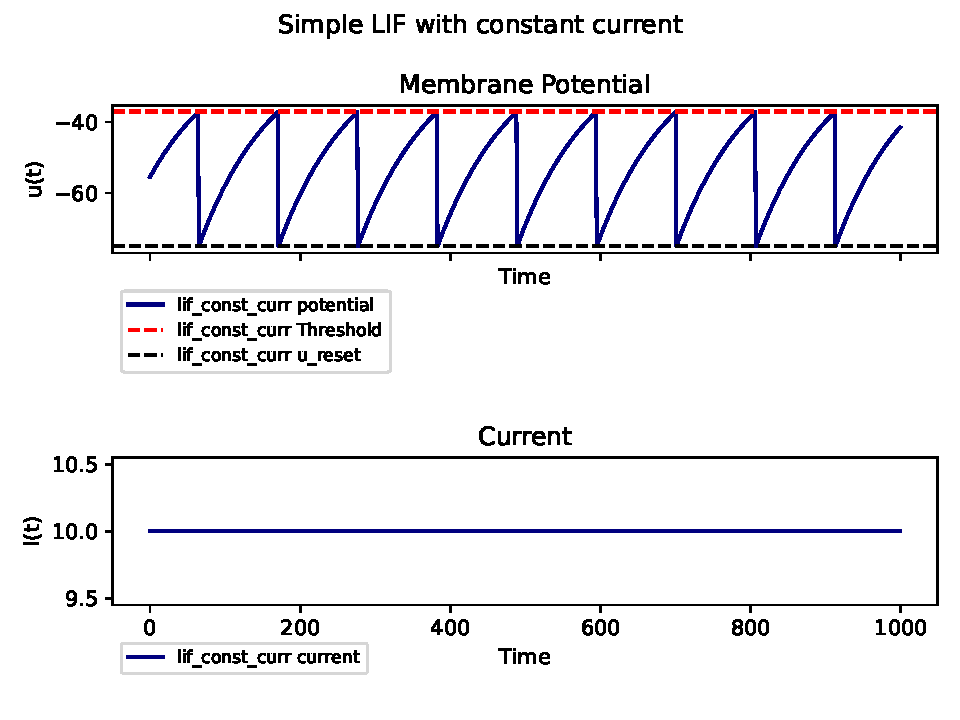
\includegraphics[width=0.8\textwidth]{plots/Simple LIF with constant current.pdf} % Include the exported plot
                \caption{مدل تجمیع و آتش نشتی با جریان ثابت.}
                \label{fig:lif-const-curr}
            \end{figure}

            حال بیاییم برخی پارامتر های مدلمان را تغییر دهیم تا تاثیر آن ها را مشاهده کنیم. اینکار را برای سه جریان متفاوت خیلی کم، کم و زیاد آزمایش میکنیم. همانطور که در نمودار 
            \ref{fig:lif-const-change-current-curr} 
            ملاحظه میکنید، با افزایش جریان، فرکانس ضربه ها
            ($spike$)
            بیشتر می شود و فواصل بین آن ها کم می شود.(منحنی قرمز)
            به طور عکس، کاهش کم جریان، میتواند تاثیر عکس داشته و فواصل بین ضربه ها را بیشتر کند.
            همچنین کاهش زیاد جریان سبب می شود که نورون به آستانه خود نرسد و هیچگاه ضربه نزند. این موضوع می تواند زمان استراحت نورون را که ورودی ای ندارد را توجیه کند.

            \begin{figure}[H]
                \centering
                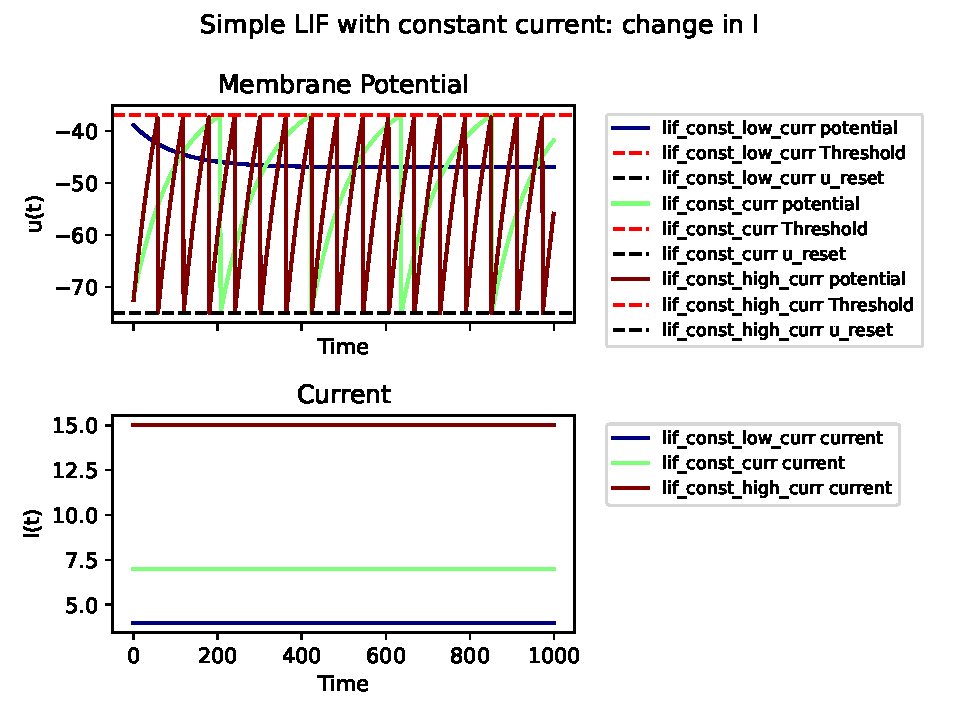
\includegraphics[width=0.8\textwidth]{plots/Simple LIF with constant current: change in I.pdf} 
                \caption{مدل تجمیع و آتش نشتی با جریان ثابت: تغییر در جریان}
                \label{fig:lif-const-change-current-curr}
            \end{figure}

            از آنجا که مدل تجمیع و آتش نشتی ساده است، تغییر پارامتر های دیگر تاثیر مشابه داشته و تنها فرکانس ضربه ها را تغییر می دهد. به طور مثال، کاهش/افزایش آستانه می تواند باعث افزایش/کاهش فرکانس ضربه ها شود.(به طور مشابه برای دیگر پارامتر ها)

            \subsubsection{جریان پله ای}
                جریان بعدی، از تابع پله ای پیروی میکند. در تابع پله ای، جریان در لحظه ای وصل شده و پس از مدت زمانی قطع می شود. پارامتر های این نمودار، کاملا مشابه جریان ثابت داده شده است و فقط در لحظات ۲۵۰ و ۷۵۰، جریان ثابت متصل می شود. در مدل تجمیع و آتش نشتی
                ($LIF$)
                لحظاتی که جریان وصل است، اختلاف پتانسیل غشای نورون مانند جریان ثابت عمل می کند. از این رو برای ما، لحظاتی که جریان وصل و قطع می شود جذاب است. همانطور که در شکل 
                \ref{fig:lif-step-curr} 
                مشاهده می شود، در ابتدای شبیه سازی، از آنجا که جریان اولیه نورون به صورت تصادفی مقدار دهی می شود، ما مقدار در حدود 
                $-65$ 
                داریم که از پتانسیل استراحت بیشتر است، پس این اختلاف پتانسیل کم کم به سمت پتانسیل استراحت یعنی 
                $-67$ 
                حرکت می کند. در لحظه ۲۵۰، جریان ثابت به نورون متصل می شود و همانطور که از نمودار پیداست، اختلاف پتانسیل غشای نورون رفته رفته بیشتر می شود تا در نهایت یک ضربه
                ($spike$)
                می زند. از این لحظه تا لحظه  ۷۵۰، رفتار نورون کاملا شبیه حالت قبل یعنی جریان ثابت می باشد. از لحظه ۷۵۰ که جریان قطع می شود، اختلاف پتانسیل نورون که تازه ضربه زده بوده و بالا می باشد، به سمت پتانسیل استراحت حرکت می کند.
                \begin{figure}[H]
                    \centering
                    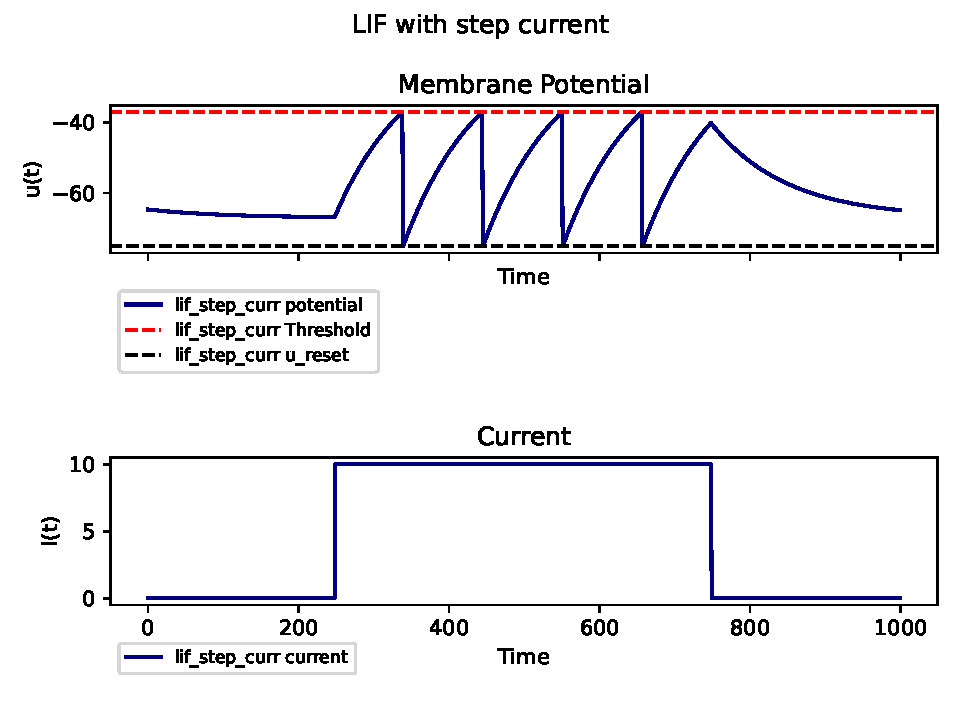
\includegraphics[width=0.8\textwidth]{plots/LIF with step current.pdf} 
                    \caption{مدل تجمیع و آتش نشتی با جریان پله ای}
                    \label{fig:lif-step-curr}
                \end{figure}
                واضح است که آزمایش این مدل با جریان پله ای و پارامتر های مختلف، نتیجه ای مشابه با جریان ثابت خواهد داشت.

            \subsubsection{جریان سینوسی}
                حال به بررسی رفتار نورون با مدل تجمیع و آتش نشتی ساده با جریان سینوسی می پردازیم. پارامتر های مدل 
                $LIF$
                مان اینجا نیز مانند قبل داده شده است.
                برای شبیه سازی جریان به صورت سینوسی نیز، از کلاس 
                \texttt{SinCurrent} 
                استفاده شده است که در آن، پارامتر های تعداد فرکانس
                ($frequency$) 
                دامنه نوسان
                ($amplitude$)
                و جابه جایی عمودی و افقی داده شده است. حال با تغییر این پارامتر ها، ما نمودار های متفاوتی از اختلاف پتانسیل خواهیم داشت. همانطور که در نمودار جریان ثابت دیدیم(ودر جریان شیب دار مشاهده خواهیم کرد)، جریان مورد نیاز برای برانگیخته کردن نورون مان با پارامتر های داده شده، در حدود 
                $6$ 
                می باشد. پس مدلمان را با مقادیر متفاوتی از جریان سینوسی بر این اساس آزمایش میکنیم.
                \begin{figure}[H]
                    \centering
                    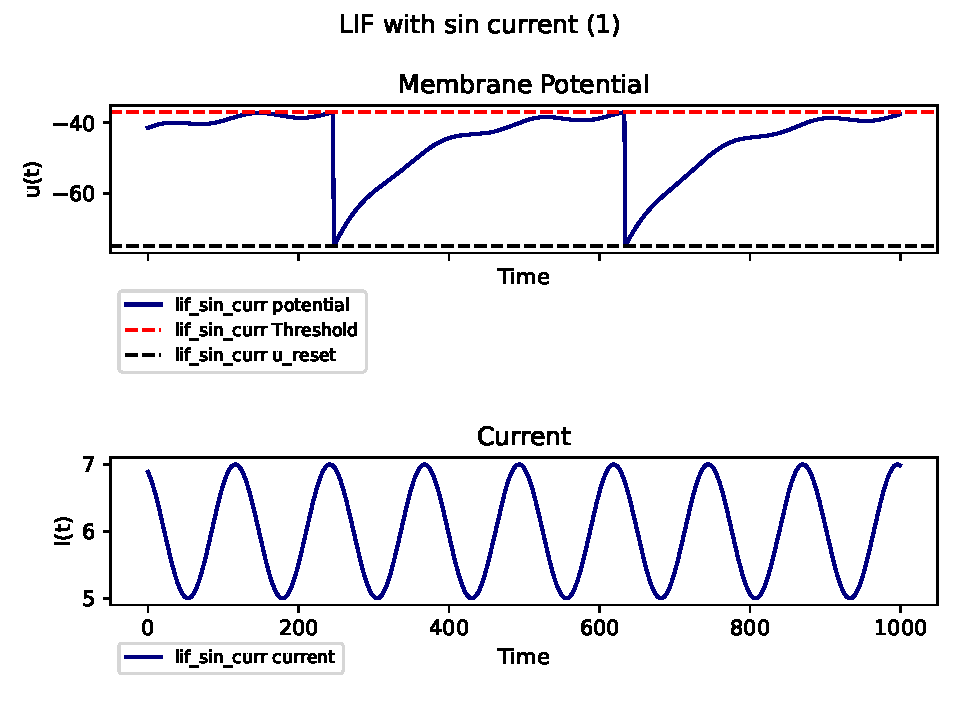
\includegraphics[width=0.8\textwidth]{plots/LIF with sin current (1).pdf} 
                    \caption{مدل تجمیع و آتش نشتی با جریان سینوسی}
                    \label{fig:lif-sin-curr}
                \end{figure}
                همانطور که ملاحظه می کنید، اگر عرض از مبدا نمودار سینوسی را در حدود 
                $6$ 
                قرار داده و دامنه نوسان را یک بگذاریم، نمودار مشابه نمودار جریان ثابت می شود با این تفاوت که چون حول جریان 
                $6$ 
                نوسان میکند(ولی نه خیلی زیاد و نه خیلی کم می شود)
                روی نمودار اختلاف پتانسیل نیز نوسان ایجاد می شود.
                اگر با همین عرض از مبدا، دامنه نوسان را نیز افزایش دهیم، صرفا نوسان های روی نمودار اختلاف پتانسیل زیاد می شود و اگر دامنه نوسان را خیلی بیشتر کنیم، نوسان های روی اختلاف پتانسیل نیز آنقدر زیاد شده تا خود نیز به آستانه نورون رسیده و در نهایت تعداد ضربه ها بیشتر می شود.
                (شکل \ref{fig:lif-sin-amp-change-curr})

                \begin{figure}[H]
                    \centering
                    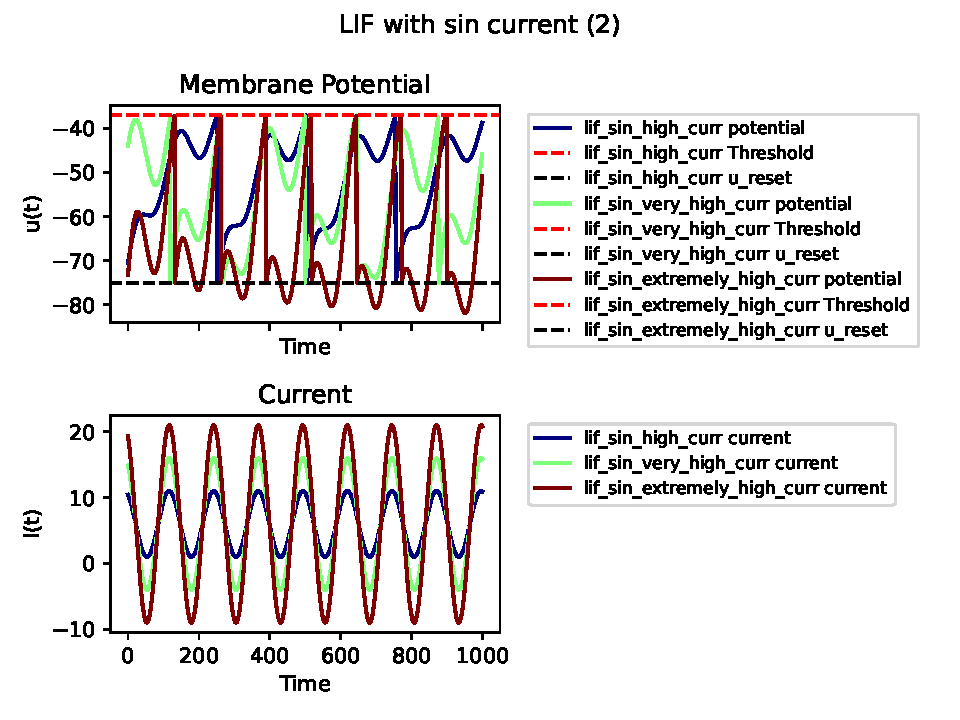
\includegraphics[width=0.8\textwidth]{plots/LIF with sin current (2).pdf} 
                    \caption{مدل تجمیع و آتش نشتی با جریان های سینوسی}
                    \label{fig:lif-sin-amp-change-curr}
                \end{figure}

                لازم به ذکر است که تاثیر پارامتر 
                $frequency$ 
                نیز روی فاصله ضربه ها و نوسانات روی نمودار اختلاف پتانسیل تاثیر دارد.
                (شکل \ref{fig:lif-sin-high-freq-curr})
                \begin{figure}[H]
                    \centering
                    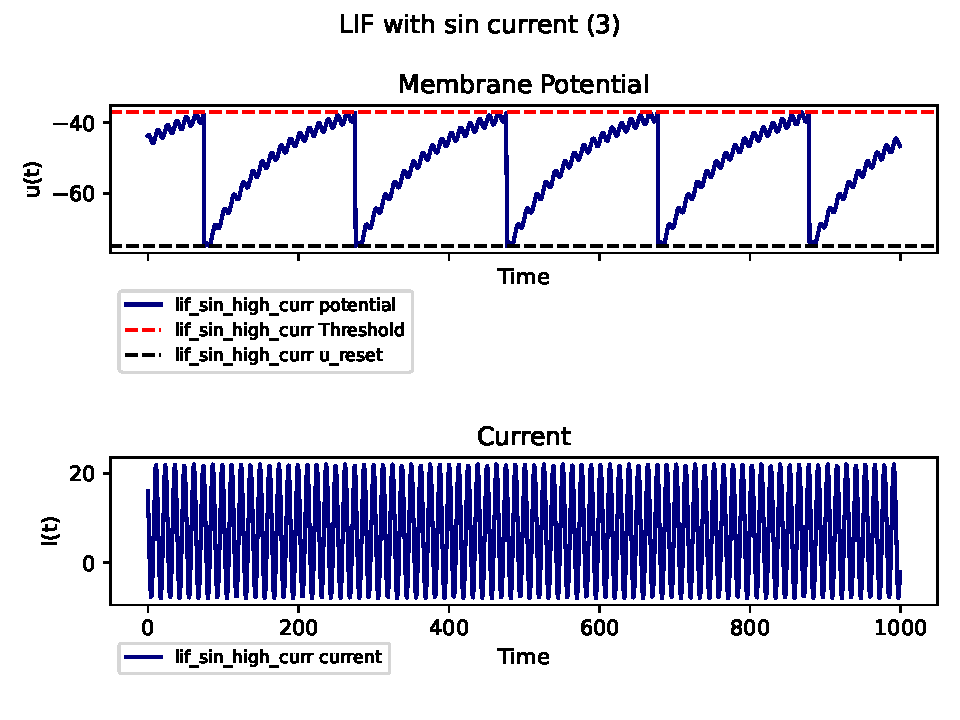
\includegraphics[width=0.8\textwidth]{plots/LIF with sin current (3).pdf} 
                    \caption{مدل تجمیع و آتش نشتی با جریان سینوسی فرکانس بالا}
                    \label{fig:lif-sin-high-freq-curr}
                \end{figure}

            \subsubsection{جریان شیب دار}
                در این نوع تابع، جریان به صورت تدریجی با یک شیب ثابت افزایش می یابد. همانطور که از نمودار
                \ref{fig:lif-ramp-curr}
                نیز مشخص است، مطابق انتظار، از جایی به بعد
                (جریان $6$) 
                که جریان مناسب برای ضربه
                ($spik$) 
                زدن فراهم می شود، صرفا فرکانس ضربه ها افزایش می یابد و با فواصل کمتری رخ می دهند.
                 
                \begin{figure}[H]
                    \centering
                    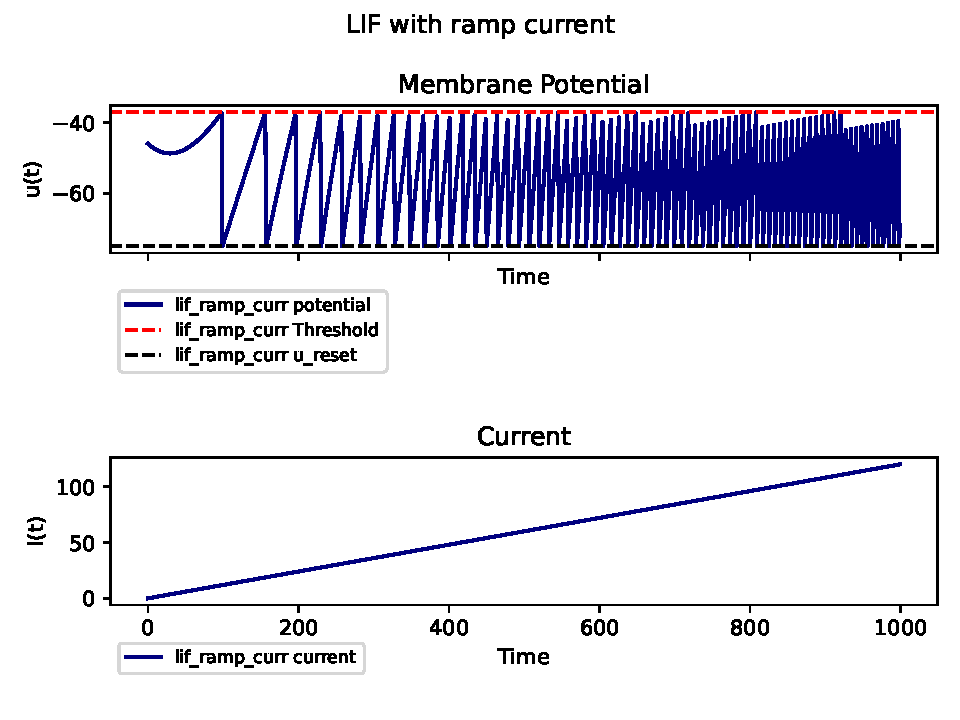
\includegraphics[width=0.8\textwidth]{plots/LIF with ramp current.pdf} 
                    \caption{مدل تجمیع و آتش نشتی با جریان شیب دار}
                    \label{fig:lif-ramp-curr}
                \end{figure}
                از آنجا که در این روش جریان یک نمودار خطی است، تغیر در شیب جریان یا عرض از مبدا آن، صرفا می تواند فرکانس ضربه ها را کمتر یا بیشتر کند.
            \subsubsection{جریان لگاریتمی}
                از آنجا که جریان، لگاریتمی، بعد از زمانی تقریبا نزدیک به یک جریان ثابت می شود، انتظار داریم که بعد از مدتی همانند نمودار جریان ثابت رفتار کند که این موضوع از روی نمودار 
                \ref{fig:lif-log-curr}
                قابل مشاهده است.
                \begin{figure}[H]
                    \centering
                    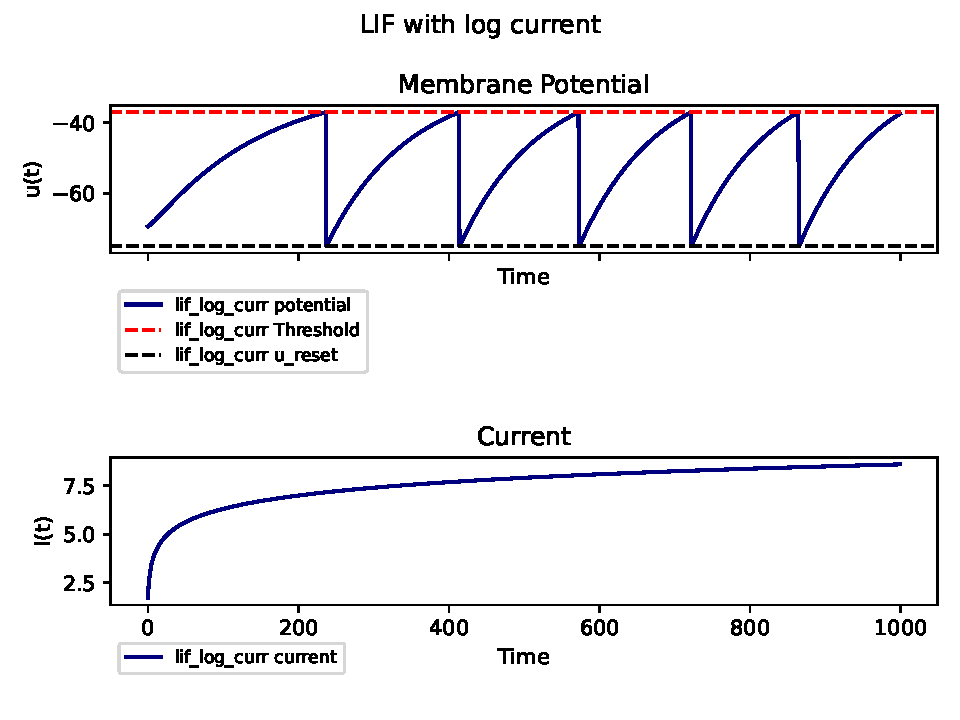
\includegraphics[width=0.8\textwidth]{plots/LIF with log current.pdf} 
                    \caption{مدل تجمیع و آتش نشتی با جریان لگاریتمی}
                    \label{fig:lif-log-curr}
                \end{figure}
                همانطور که از نمودار نیز پیداست، در ابتدا که جریان کم می باشد، اختلاف پتانسیل نیز به آرامی افزایش پیدا می کند، و رفته رفته که نمودار به جریان مورد نیاز برای ضربه نزدیک می شود و از آن به اهستگی عبور میکند، نورون علاوه بر ضربه زدن، فرکانس ضربه زدنش نیز به آرامی افزایش یافته و سپس تقریبا ثابت می شود.

                از آنجا که نمودار لگاریتمی بعد از زمانی به شدت به آرامی افزایش می یابد، تغییرات پارامتر ها در زمان زیاد، تغییر چندانی نمیگذارد و تقریبا مانند نمودار جریان ثابت می شود.

        \subsection{مدل تجمیع و آتش نشتی نمایی ($ELIF$)}
            حال به بررسی مدل تجمیع و آتش نمایی با جریان های متفاوت می پردازیم.
            \subsubsection{جریان ثابت}
                اولین جریان، جریان با مقدار ثابت می باشد. میدانیم که مدل تجمیع و آتش نشتی نمایی میتواند نسبت به مدل 
                $LIF$ 
                ساده، بالا رفتن اختلاف پتانسیل تا زمان ضربه
                ($spike$) 
                زدن را نیز شبیه سازی کند. این موضوع را میتوان از نمودار
                \ref{fig:elif-const-curr}
                با جریان ساده زیر دریافت نمود.
                برای این مدل، من از پارامتر های مدل قبلی، بجز آستانه و مقاومت که به ترتیب برابر 
                $-13$ و
                $1.7$
                استفاده کردم چرا که با در نظر گرفتن دقت زمانی 
                $0.5$
                نمودار بهتری کشیده می شد و تفاوت مهمی ندارد. همچنین در این مدل یک پارامتر جدید به نام
                $u_{rh}$ 
                نیز داریم که آستانه ای است که اگر اختلاف پتانسیل غشای نورون به آن برسد، با شیب بسیار زیاد به طور خودکار تا آستانه ضربه نورون بالا می رود. پارامتر جدید دیگر نیز، 
                $\Delta T$ می باشد که تنظیم کننده میزان تیز بودن بالا رفتن از آستانه 
                $rh$ 
                تا آستانه ضربه نورون را تنظیم می کند. میزان تاثیر این مورد را برای تفکیک بهتر در شکل، در جریان پله ای بررسی می کنیم.
                \begin{figure}[H]
                    \centering
                    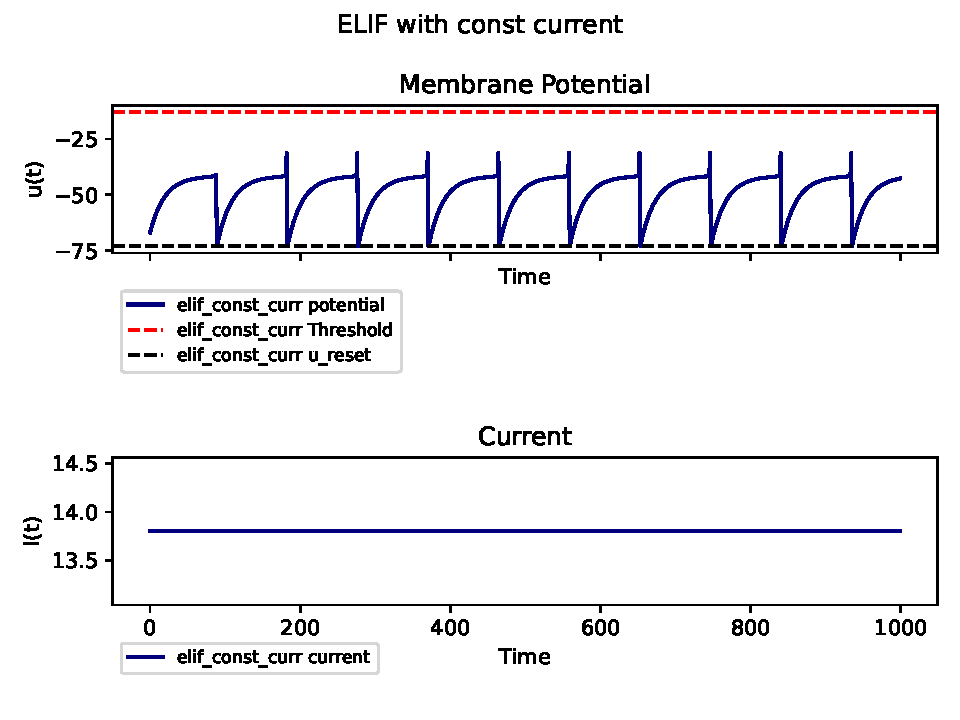
\includegraphics[width=0.8\textwidth]{plots/ELIF with const current.pdf} 
                    \caption{مدل تجمیع و آتش نشتی نمایی با جریان ثابت}
                    \label{fig:elif-const-curr}
                \end{figure}
                همانطور که در نمودار نیز ملاحظه می شود، پس از رسیدن اختلاف پتانسیل غشا به 
                $u_{rh}$ 
                اختلاف پتانسیل غشا به طور ناگهانی زیاد شده و با رسیدن به آستانه، ضربه
                ($spike$) 
                میزند. از آنجا که شیب بالا رفت این اختلاف پتانسیل بسیار بالا است، ممکن است در نمودار این بالا رفتن به خوبی نمایش داده نشود چرا که باید دقت زمانی به بسیار زیاد نمود. در این مدل نیز، کم و زیاد کردن جریان ثابت، صرفا فرکانس ضربه ها و شیب بالا رفتن اختلاف پتانسیل را می تواند زیاد کند. 
                (شکل \ref{fig:elif-const-change-curr})

                \begin{figure}[H]
                    \centering
                    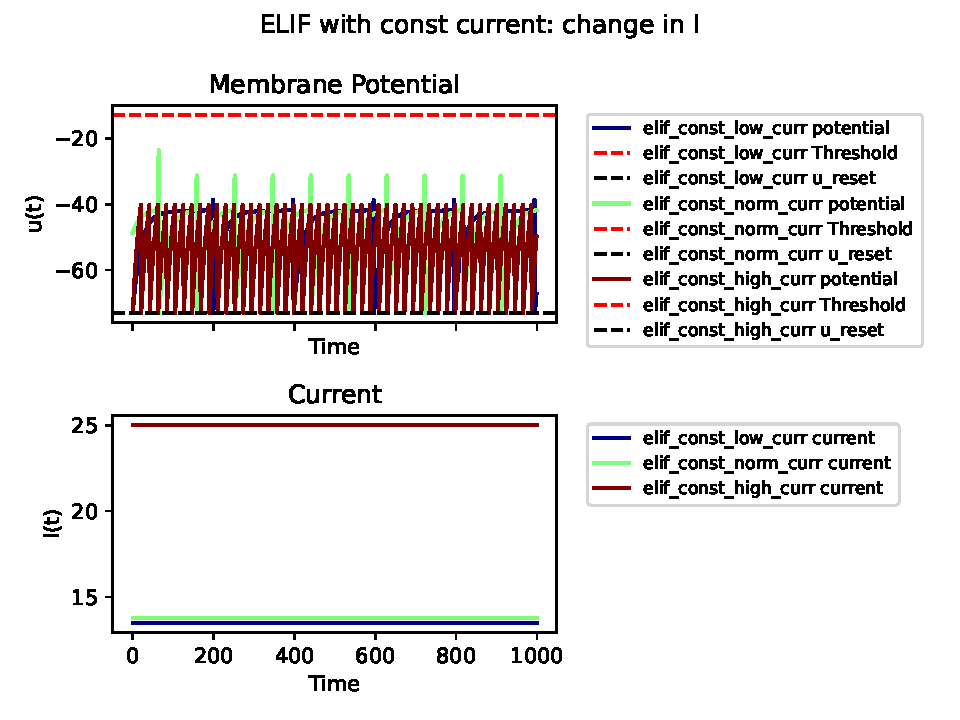
\includegraphics[width=0.8\textwidth]{plots/ELIF with const current: change in I.pdf} 
                    \caption{مدل تجمیع و آتش نشتی نمایی با جریان های ثابت متفاوت}
                    \label{fig:elif-const-change-curr}
                \end{figure}
                از آنجا که با افزایش 
                $\Delta T$ 
                و کاهش آستانه 
                $u_{rh}$ 
                می توان هم شدت افزایش خودکار تا آستانه ضربه را کاهش داد و هم طول آن را بیشتر کرد، با ترکیب این دو تغییر در پارامتر ها، میتوان تفاوت مدل 
                $ELIF$ 
                با $LIF$ 
                را به صورت لمس شدنی برای شهود بیشتر نمایش داد.
                (شکل \ref{fig:elif-const-curr-change-rh-T})
                \begin{figure}[H]
                    \centering
                    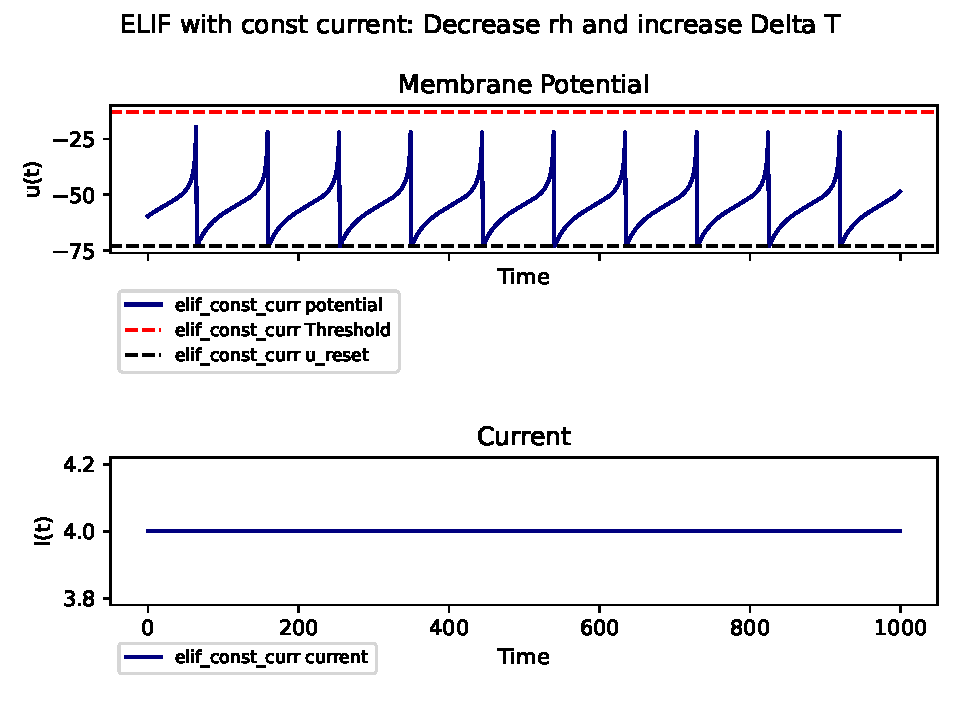
\includegraphics[width=0.8\textwidth]{plots/ELIF with const current: Decrease rh and increase Delta T.pdf} 
                    \caption{مدل تجمیع و آتش نشتی نمایی با جریان ثابت: کاهش $u_{rh}$ و افزایش $\Delta T$}
                    \label{fig:elif-const-curr-change-rh-T}
                \end{figure}

            \subsubsection{جریان پله ای}
                از آنجا که مدل تجمیع و آتش نشتی نمایی، تنها بالا رفتن تا سطح آستانه را علاوه بر مدل ساده، شبیه سازی میکند، انتظار داریم که تغییرات مشابهی را که با جریان پله ای در مدل ساده دیدیم در آن مشاهده کنیم. نمودار
                \ref{fig:elif-step-curr}
                گواه این ادعا است.
                \begin{figure}[H]
                    \centering
                    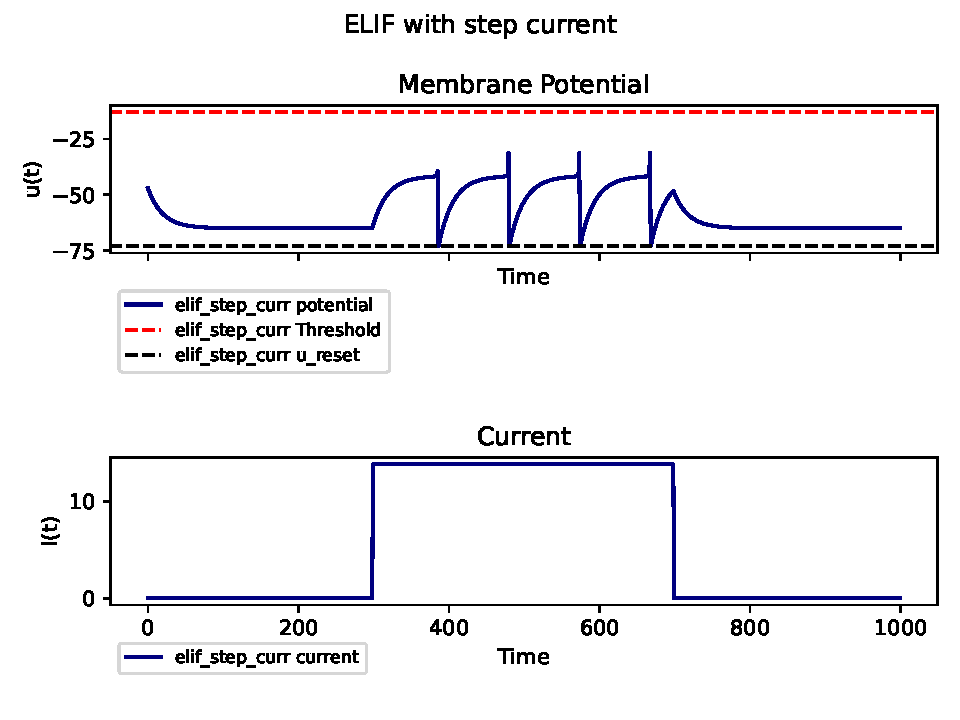
\includegraphics[width=0.8\textwidth]{plots/ELIF with step current.pdf} 
                    \caption{مدل تجمیع و آتش نشتی نمایی با جریان پله ای }
                    \label{fig:elif-step-curr}
                \end{figure}
                واضح است که آزمایش این مدل با جریان پله ای و پارامتر های مختلف، نتیجه ای مشابه با جریان ثابت خواهد داشت.
                تنها پارامتر باقی مانده برای بررسی که پیشتر آن را در جریان ثابت بررسی کردیم، پارامتر
                $\Delta T$ 
                است که تغییرات آن در شکل 
                \ref{fig:elif-step-curr-change-T}
                نمایش داده شده است.
                \begin{figure}[H]
                    \centering
                    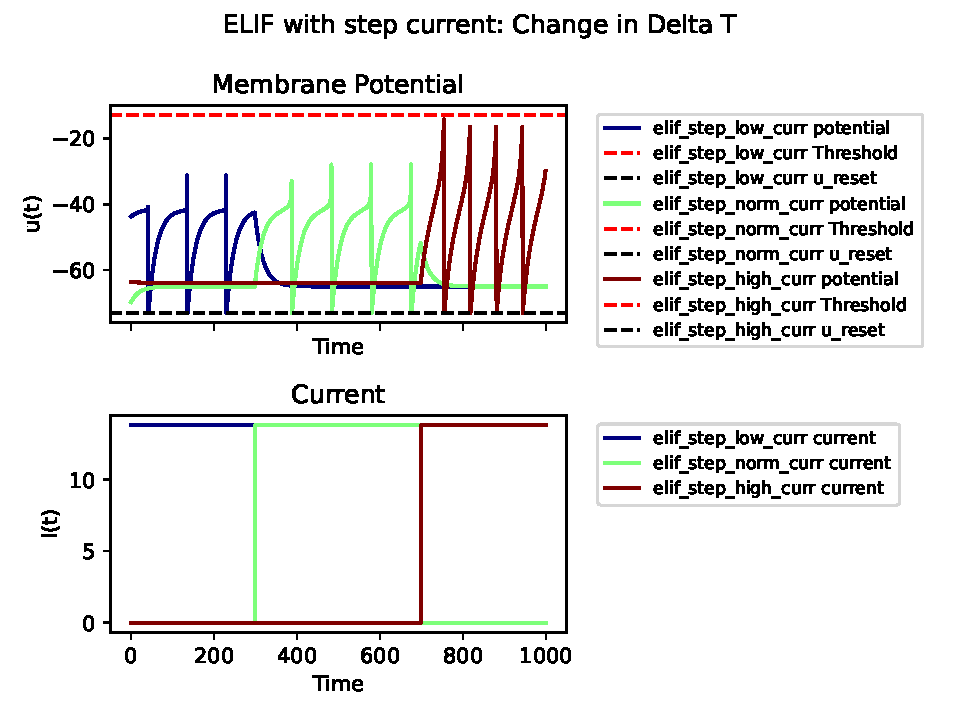
\includegraphics[width=0.8\textwidth]{plots/ELIF with step current: Change in Delta T.pdf} 
                    \caption{مدل تجمیع و آتش نشتی نمایی با جریان پله ای: تغییر در $\Delta T$}
                    \label{fig:elif-step-curr-change-T}
                \end{figure}
            \subsubsection{جریان سینوسی}
                تاثیر جریان سینوسی بر مدل تجمیع و آتش نشتی نمایی نیز همانند تاثیر آن بر مدل تجمیع و آتش نشتی ساده است و تنها تفاوت، همان بالا رفتن ناگهانی و خودکار اختلاف پتانسیل غشا پس از رسیدن به 
                $u_{rh}$ 
                می باشد.
                (شکل \ref{fig:elif-sin-curr})
                تغییر در پارامتر های 
                $\Delta T$ یا
                $u_{rh}$ 
                نیز مانند جریان های قبلی است.
                \begin{figure}[H]
                    \centering
                    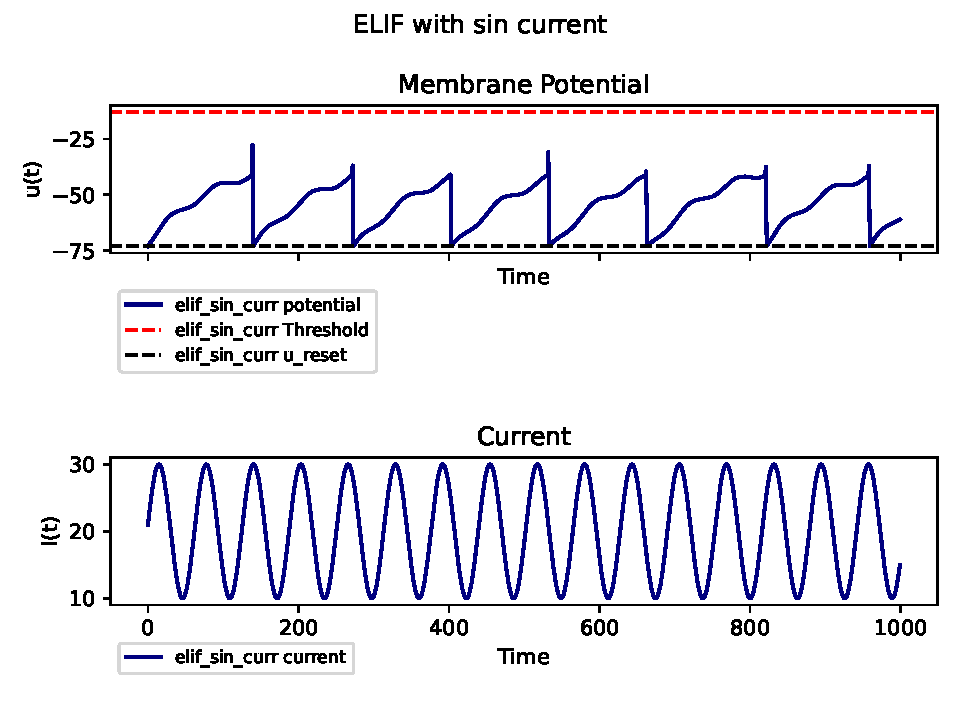
\includegraphics[width=0.8\textwidth]{plots/ELIF with sin current.pdf} 
                    \caption{مدل تجمیع و آتش نشتی نمایی با جریان سینوسی}
                    \label{fig:elif-sin-curr}
                \end{figure}

            \subsubsection{جریان شیب دار}
                به طور مجدد، استفاده از جریان شیبدار، تاثیر مشابهی که روی 
                $LIF$ 
                گذاشت را روی مدل 
                $ELIF$ 
                خواهد داشت. یعنی با افزایش تدریجی با شیب ثابت جریان، فرکانس ضربه های نورون نیز افزایش خواهد یافت.
                (شکل \ref{fig:elif-ramp-curr})
                \begin{figure}[H]
                    \centering
                    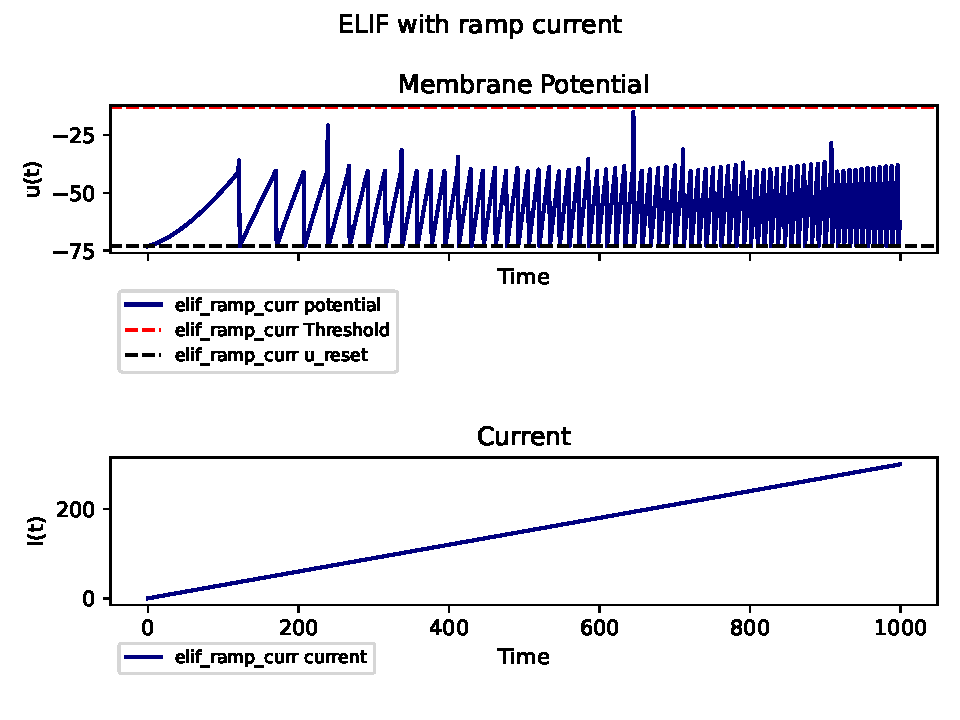
\includegraphics[width=0.8\textwidth]{plots/ELIF with ramp current.pdf} 
                    \caption{مدل تجمیع و آتش نشتی نمایی با جریان شیبدار}
                    \label{fig:elif-ramp-curr}
                \end{figure}

            \subsubsection{جریان لگاریتمی}
                نیازی به ذکر مجدد این موضوع نیست که در تابع لگاریتمی هر چه به سمت بی نهایت می رویم، شیب تغییرات آن به شدت کاهش یافته به طوری که تقریبا مانند یک تابع با مقدار ثابت می شود. هر چند که شیب تغییرات آن در ابتدا نسبتا زیاد است. از این رو، تاثیر این نوع جریان روی اختلاف پتانسیل در ابتدا زیاد، و پس از مدتی کاهش می یابد.
                (شکل \ref{fig:elif-ramp-curr})
                \begin{figure}[H]
                    \centering
                    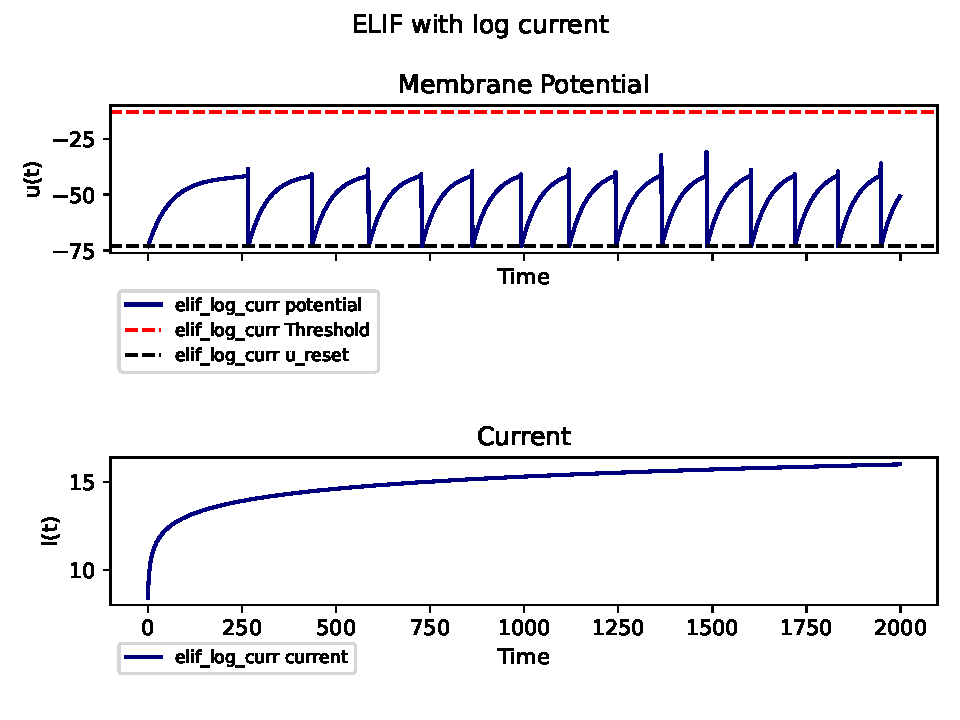
\includegraphics[width=0.8\textwidth]{plots/ELIF with log current.pdf} 
                    \caption{مدل تجمیع و آتش نشتی نمایی با جریان لگاریتمی}
                    \label{fig:elif-ramp-curr}
                \end{figure}

        \subsection{مدل تجمیع و آتش نشتی نمایی تطبیق پذیر ($AELIF$)}
            نوبت به آخرین مدل از این قسمت از پروژه می رسد، یعنی مدل تجمیع و آتش نشتی نمایی تطبیق پذیر
            ($AELIF$).
            این مدل نسبت به دو مدل قبلی، می تواند اطلاعات بیشتری را شبیه سازی کند. به عبارت دیگر، این مدل می تواند الگو های ضربه
            ($spike$) 
            بیشتری را مدل کند. اینکار توسط یک سری معادله دیفرانسیل دیگر انجام می شود که میتوانند فرایند تطبیق پذیری
            ($adaptation$) 
            را شبیه سازی کند. معادله کلی این مدل، با در نظر گرفتن یک تطبیق پذیری به صورت زیر است:
            \begin{latin}
                \begin{equation}
                    \tau_m.\frac{du}{dt} = - (u - u_{rest}) + \Delta_T exp(\frac{u - \theta_{rh}}{\Delta_T}) - Rw + R.I(t)
                \end{equation}
                \begin{equation}
                    \tau_w.\frac{dw}{dt} = a(u - u_{rest}) - w + b\tau_w\Sigma_{t^{f}}\delta(t-t^f)
                \end{equation}
            \end{latin}
            در این مدل نیز، به طور مشابه باید کاری را که برای محاسبه 
            $u$ 
            در هر مرحله براساس 
            $du$ 
            انجام میدادیم را برای محاسبه 
            $w$ 
            نیز انجام دهیم. پیاده سازی اینکار، توسط تابع زیر در کد ها انجام شده است:
            \begin{latin}
                \centering
                \begin{lstlisting}[language=Python]
def update_w(self, ng):
    leakage = ng.u - self.u_rest
    ng.w += ((self.a * leakage - ng.w + self.b * self.tau_w * \
            ng.spike.byte()) / self.tau_w) * ng.network.dt
                \end{lstlisting}
            \end{latin}
            در ابتدا یک توضیح کلی درمورد هر یک از پارامتر های جدیدی که اضافه شده است می دهیم و سپس به بررسی مدل با جریان های مختلف می رویم تا هنگاه آزمون پارامتر های مختلف، دچار سردرگمی نشویم.

            متغیری که نسبت به مدل های قبلی در این مدل اضافه شده است، متغیر 
            $w$ 
            است که وابسته به پارامتر های 
            $a$, 
            $b$ و 
            $\tau_w$
            است.

            پارامتر 
            $a$ 
            نیروی اتصال بین جریان تطبیقی و پتانسیل غشایی است. این پارامتر مشخص می‌کند چه مقدار جریان تطبیقی بر پتانسیل غشایی تأثیر می‌گذارد. به طور ساده تر، این پارامتر میزان حساسیت به اختلاف پتانسیل را تنظیم می کند.

            پارامتر 
            $b$ 
            نشان دهنده حلقه بازخورد مثبت در دینامیک نورون است، جایی که فعالیت اسپایکی منجر به افزایش جریان تطبیقی می‌شود که به نوبه خود تأثیرگذاری بر تحریک‌پذیری نورون را دارد. به طور ساده تر، این پارامتر میزان مقاومت نورون نسبت به جریان را نسبت به ضربه هایی که زده شده است را تعیین می کند.

            حال با بررسی نمودار های مختلف، تاثیر تابع جریان و پارامتر های مختلف را بر این مدل مشاهده می کنیم.
            \subsubsection{جریان ثابت}
                طبق چیزی که از تعریف مدل تطبیق پذیر انتظار داریم، این است که اگر یک جریان ثابت به نورون ما وارد شود، پس از چند ضربه
                ($spike$) 
                مدل ما نسبت به آن تطبیق یابد و یا با آن شدت جریان ضربه نزند یا فرکانس ضربه ها کاهش یابد.(بسته به الگوی ضربه مورد نظر) این مورد را میتوان به وضوح از نمودار 
                \ref{fig:aelif-const-curr} 
                دریافت کرد.
                در این مدل، پارامتر ها به صورت 
                $a=6.7$, 
                $b=0.01$, 
                $R=1.7$, 
                $tau_m=10$, 
                $tau_w=100$, 
                $threshold=-30$, 
                $u_{rh}=-50$, 
                $u_{rest}=-65$, 
                $u_{reset}=-70$, 
                $Delta_T=1$
                است. 
                \begin{figure}[H]
                    \centering
                    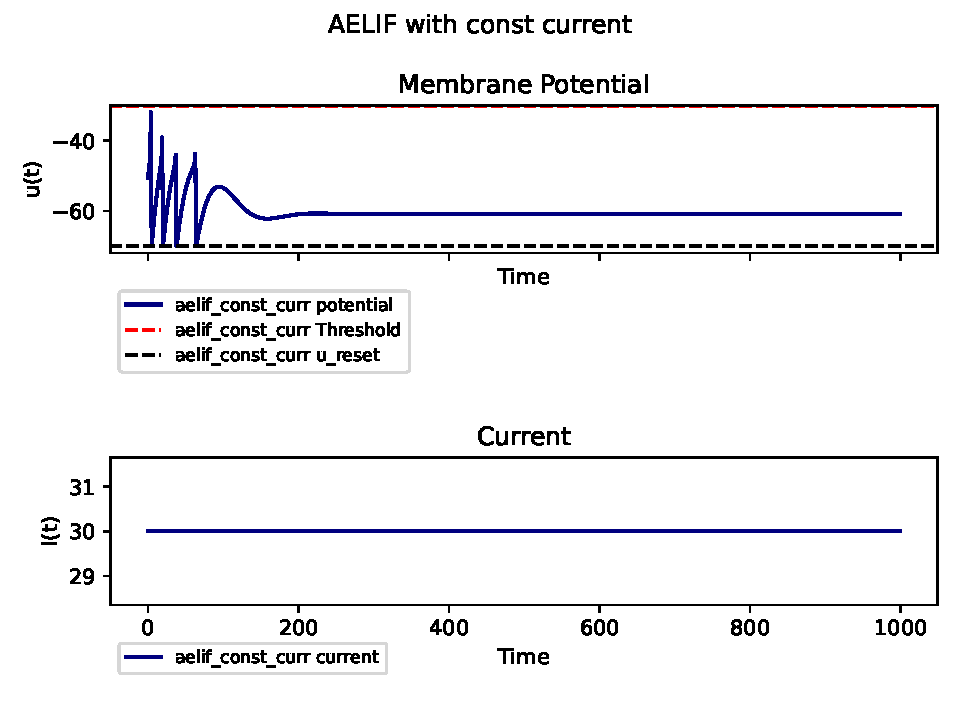
\includegraphics[width=0.8\textwidth]{plots/AELIF with const current.pdf} 
                    \caption{مدل تجمیع و آتش نشتی نمایی تطبیق پذیر با جریان ثابت}
                    \label{fig:aelif-const-curr}
                \end{figure}
                
                همانطور که ملاحظه می شود، در ابتدا که جریان تازه به نورون وارد شده است، نورون شروع به ضربه زدن می کند و پس از مدتی نسبت به این جریان ثابت مقاوم شده و نه تنها فرکانس ضربه ها کاهش می یابد، بلکه دیگر این جریان به راحتی نورون را برانگیخته نمی کند.
                نمودار تغییرات 
                $w$ 
                نسبت به زمان نیز در شکل 
                \ref{fig:aelif-w-const-curr}
                نشان داده شده است.
                \begin{figure}[H]
                    \centering
                    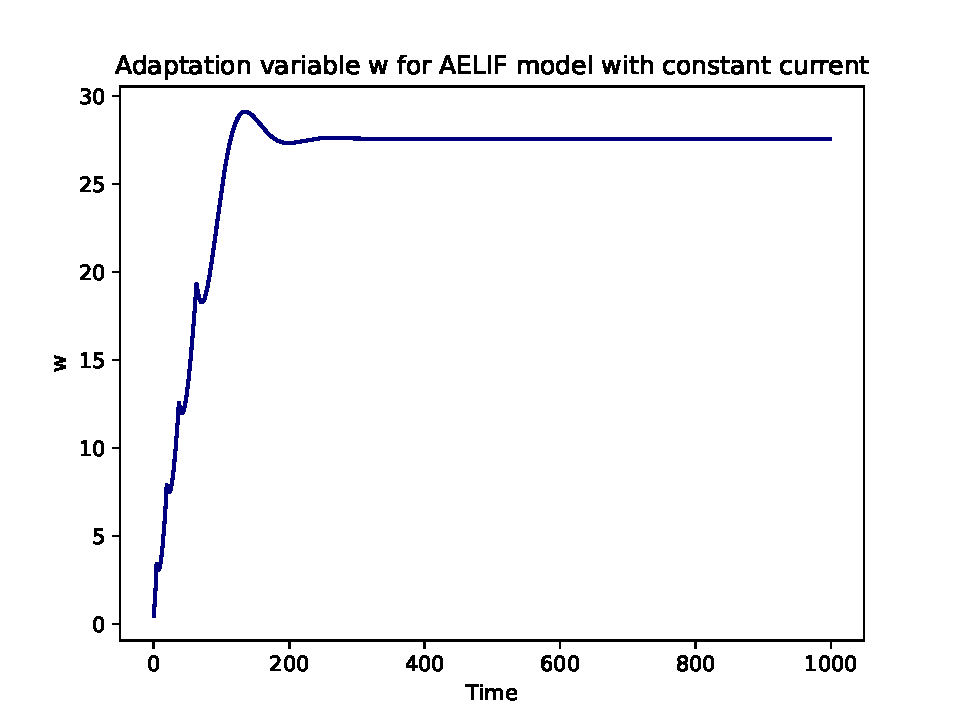
\includegraphics[width=0.8\textwidth]{plots/Adaptation variable w for AELIF model with constant current.pdf} 
                    \caption{تغییرات $w$ در مدل تجمیع و آتش نشتی نمایی تطبیق پذیر با جریان ثابت}
                    \label{fig:aelif-w-const-curr}
                \end{figure}
                
                حال اگر جریان را زیاد کنیم چه اتفاقی می افتد؟ انتظار داریم که این تطبیق پذیری در زمان بیشتری تأثیر خود را روی نورون بگذارد و به عبارت دیگر، نورون دیرتر به محرک مقاوم شود. این موضوع از نمودار
                \ref{fig:aelif-high-const-curr} و
                \ref{fig:aelif-w-high-const-curr}
                دریافت می شود.
                \begin{figure}[H]
                    \centering
                    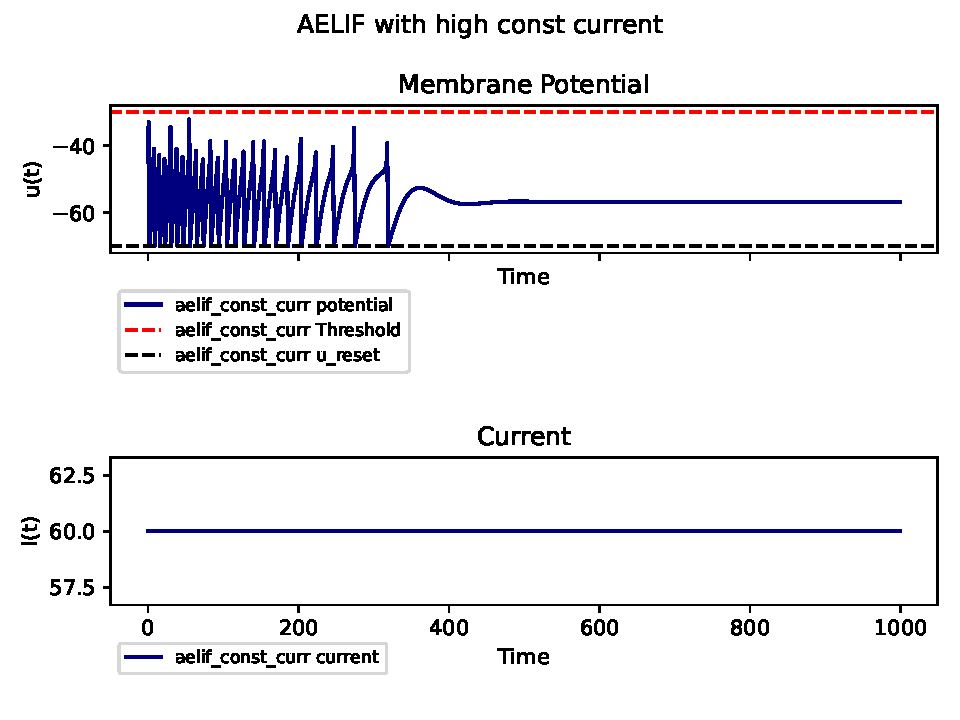
\includegraphics[width=0.8\textwidth]{plots/AELIF with high const current.pdf} 
                    \caption{مدل تجمیع و آتش نشتی نمایی تطبیق پذیر با جریان ثابت}
                    \label{fig:aelif-high-const-curr}
                \end{figure}
                \begin{figure}[H]
                    \centering
                    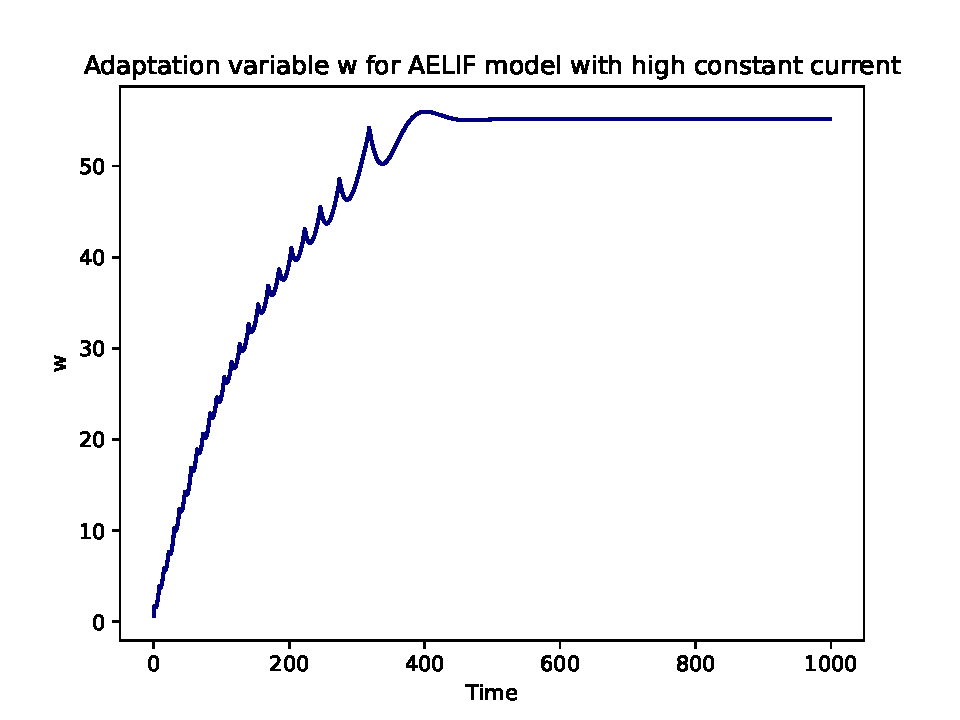
\includegraphics[width=0.8\textwidth]{plots/Adaptation variable w for AELIF model with high constant current.pdf} 
                    \caption{تغییرات $w$ در مدل تجمیع و آتش نشتی نمایی تطبیق پذیر با جریان ثابت زیاد}
                    \label{fig:aelif-w-high-const-curr}
                \end{figure}
                تغییر در متغیر 
                $\tau_w$ 
                منجر به چه چیزی می شود؟ این مورد را با سه مقدار در اندازه های مختلف آزمایش می کنیم.
                همانطور که از تعریف و نمودار
                \ref{fig:aelif-const-curr-change-tau_w} و 
                \ref{fig:aelif-w-const-curr-change-tau_w}
                پیداست، این پارامتر، حساسیت نورون و تطبیق پذیری آن را نسبت به زمان تعیین میکند. به طوری که مقدار کم آن حساسیت زیاد و مقدار زیاد آن حساسیت کم ایجاد می کند. به عنوان مثال، با قرار دادن 
                $tau_w=400$، 
                میبینیم که نسب به 
                $tau_w=1$ 
                بسیار دیر تر تطبیق می یابد.
                \begin{figure}[H]
                    \centering
                    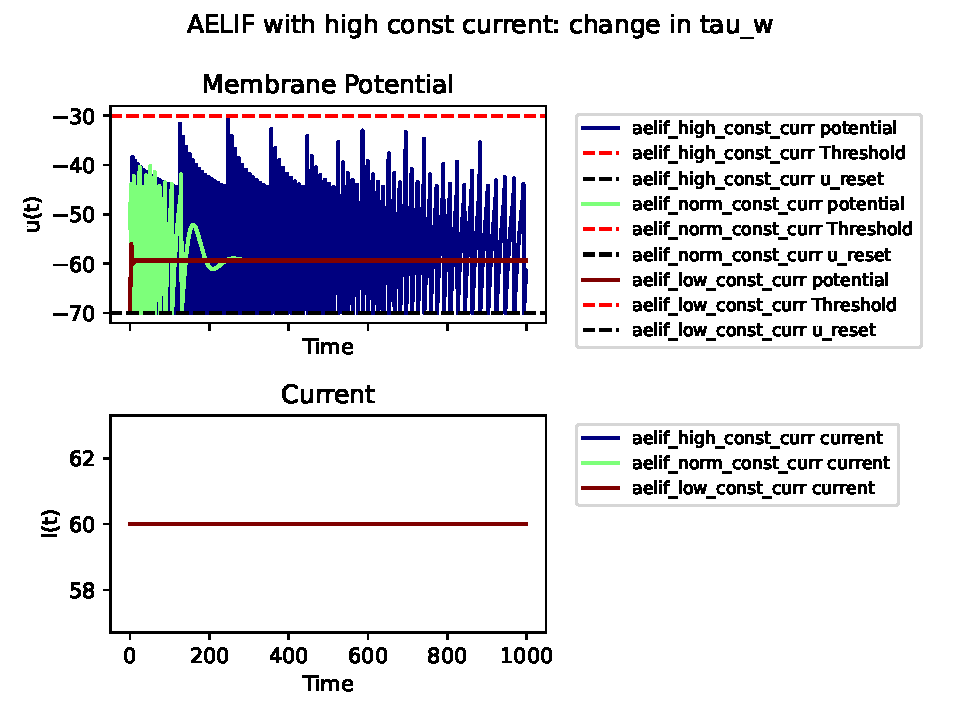
\includegraphics[width=0.8\textwidth]{plots/AELIF with high const current: change in tau_w.pdf} 
                    \caption{مدل تجمیع و آتش نشتی نمایی تطبیق پذیر با جریان ثابت: تغییر در $\tau_w$}
                    \label{fig:aelif-const-curr-change-tau_w}
                \end{figure}
                \begin{figure}[H]
                    \centering
                    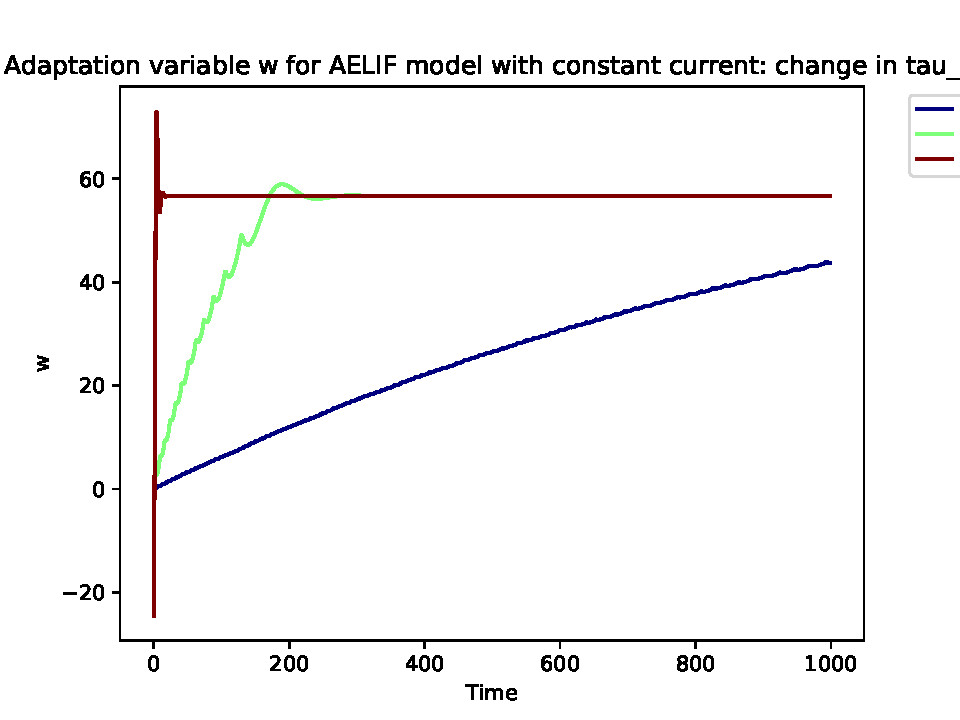
\includegraphics[width=0.8\textwidth]{plots/Adaptation variable w for AELIF model with constant current: change in tau_w.pdf} 
                    \caption{تغییرات $w$ در مدل تجمیع و آتش نشتی نمایی تطبیق پذیر با جریان ثابت: تغییر در $\tau_w$}
                    \label{fig:aelif-w-const-curr-change-tau_w}
                \end{figure}
            \subsubsection*{جریان پله ای}
                در جریان پله ای نیز انتظار داریم که نمودار پس از لحظه 
                $t_0$ 
                نیز مانند نمودار جریان ثابت رفتار کند و در واقع همین اتفاق نیز می افتد.
                (شکل \ref{fig:aelif-step-curr} و
                \ref{fig:aelif-w-step-curr})
                \begin{figure}[H]
                    \centering
                    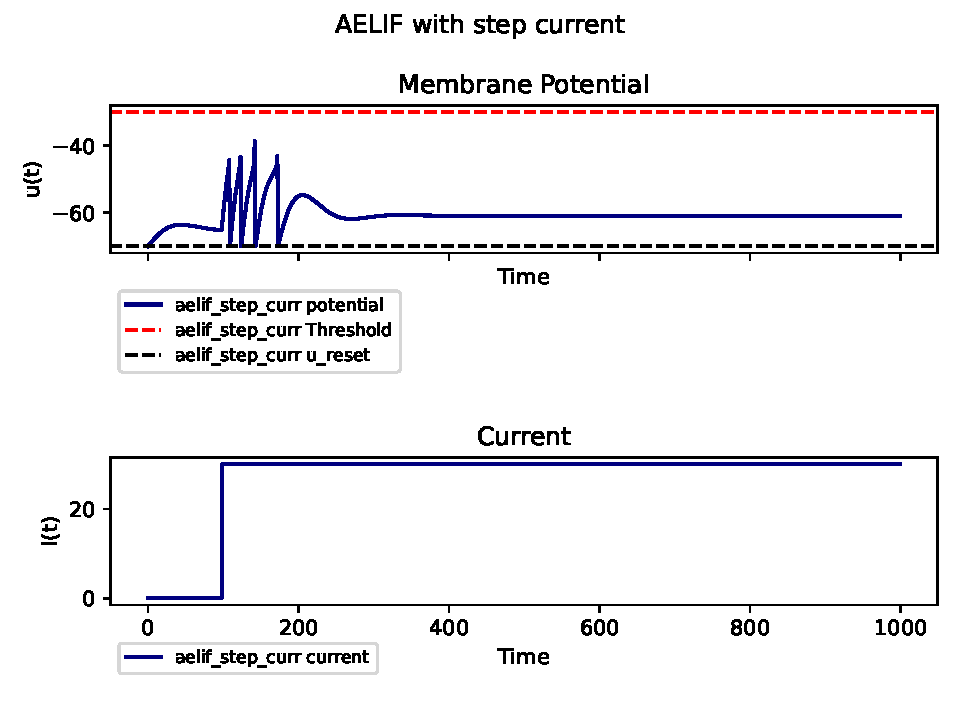
\includegraphics[width=0.8\textwidth]{plots/AELIF with step current.pdf} 
                    \caption{مدل تجمیع و آتش نشتی نمایی تطبیق پذیر با جریان پله ای}
                    \label{fig:aelif-step-curr}
                \end{figure}
                \begin{figure}[H]
                    \centering
                    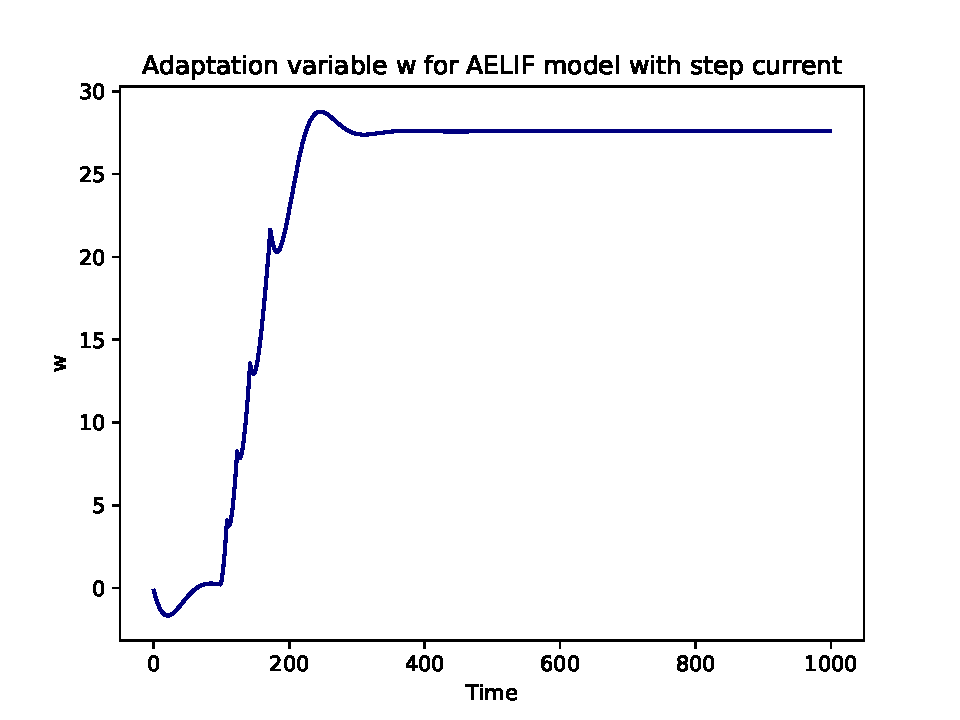
\includegraphics[width=0.8\textwidth]{plots/Adaptation variable w for AELIF model with step current.pdf} 
                    \caption{تغییرات $w$ در مدل تجمیع و آتش نشتی نمایی تطبیق پذیر با جریان پله ای}
                    \label{fig:aelif-w-step-curr}
                \end{figure}
                واضح است که تغییرات اعمال شده در پارامتر ها، نتیجه ای مشابه با تغییرات پارامتر ها در جریان ثابت را خواهد داشت.

            \subsubsection{جریان سینوسی}
                در جریان سینوسی نیز انتظار داریم که تطبیق پذیری مانند دو جریان قبلی صورت گیرد. همچنین انتظار داریم شکل ضربه زدن نورون ها نیز همانند مدل 
                $ELIF$ 
                باشد. نمودار 
                \ref{fig:aelif-sin-curr} و 
                \ref{fig:aelif-w-sin-curr}
                این موضوع را تایید می کند. تنها تفاوتی که میتوان در این جریان با جریان های قبلی پیدا کرد این است که فرایند تطبیق پذیری دیرتر اتفاق می افتاد که ممکن است به دلیل این باشد که جریان همیشه زیاد نبوده و کم و زیاد می شود
                (حدس من این است که پیچیدگی این جریان نسبت جریان های قبلی بیشتر است و نورون سخت تر به ان تطبیق می یابد. اگر در واقعیت نیز این موضوع را در نظر بگیریم، گوش ما به یک صدای ثابت و یکنواخت راحت تر تطبیق می یابد تا یک صدا که مرتبطا کم و زیاد می شود.)
                \begin{figure}[H]
                    \centering
                    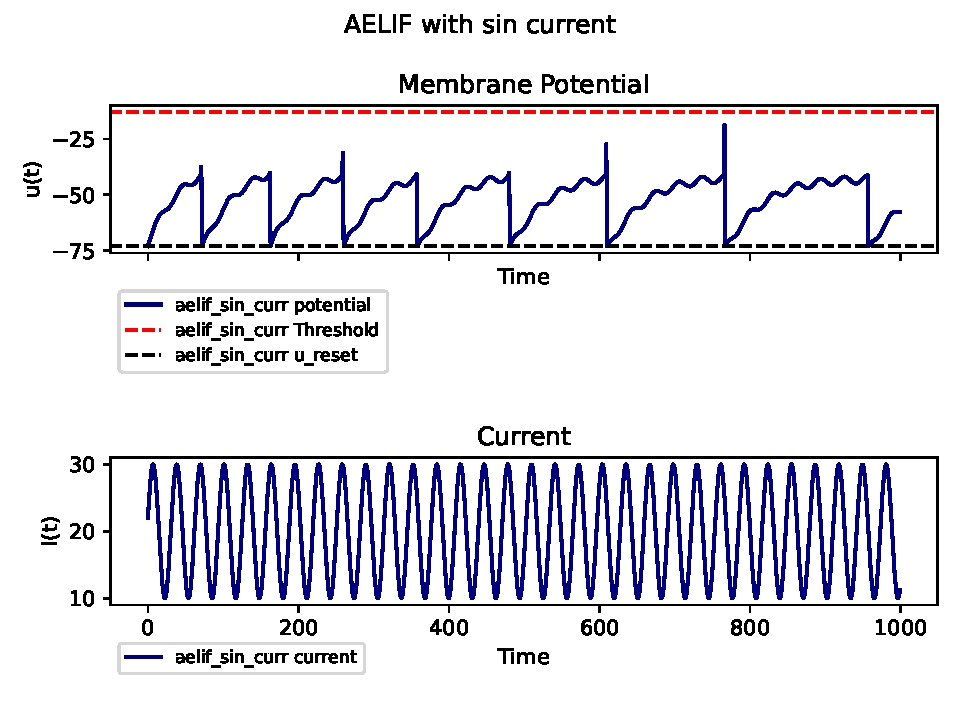
\includegraphics[width=0.8\textwidth]{plots/AELIF with sin current.pdf} 
                    \caption{مدل تجمیع و آتش نشتی نمایی تطبیق پذیر با جریان سینوسی}
                    \label{fig:aelif-sin-curr}
                \end{figure}
                \begin{figure}[H]
                    \centering
                    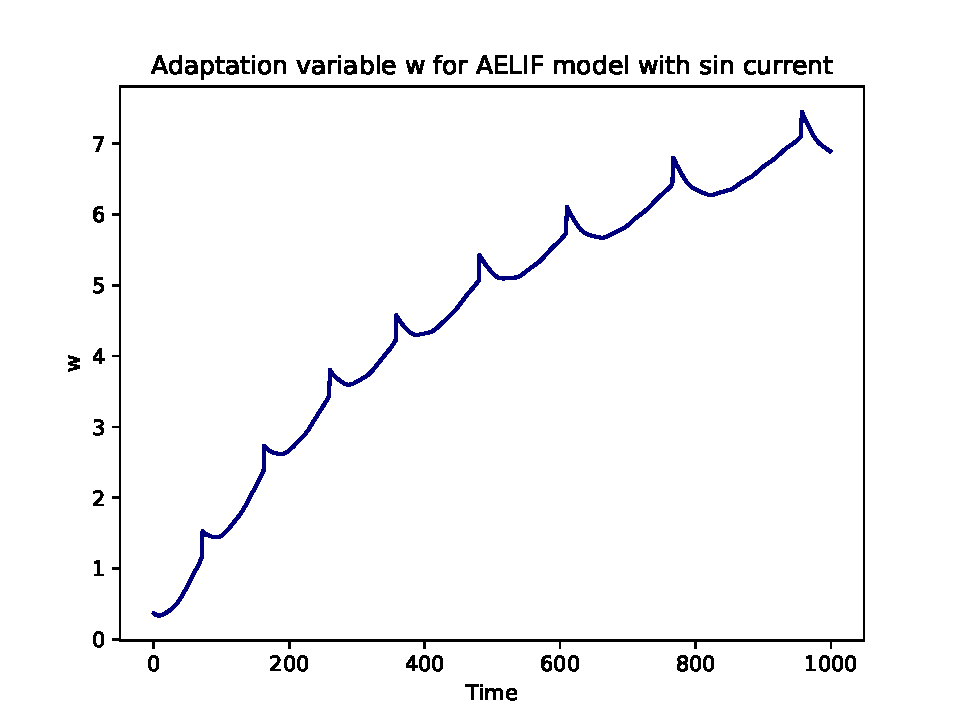
\includegraphics[width=0.8\textwidth]{plots/Adaptation variable w for AELIF model with sin current.pdf} 
                    \caption{تغییرات $w$ در مدل تجمیع و آتش نشتی نمایی تطبیق پذیر با جریان سینوسی}
                    \label{fig:aelif-w-sin-curr}
                \end{figure}
                مجددا با تغییر پارامتر ها، نتیجه یا الگوی جدیدی نسبت به تغییراتی که در جریان ها و مدل های قبلی دادیم حاصل نشد.
            \subsubsection{جریان شیب دار}
                در جریان شیب دار، به دلیل اینکه جریان ورودی به نورون مرتبط بیشتر می شود، تلاش نورون برای تطبیق کردن خود با وضعیت با شکست رو به رو می شود. در واقع همانطور که از نمودار 
                \ref{fig:aelif-ramp-curr}
                به نظر میرسد که شیب تطبیق پذیری نورونی از تابع درجه یک کمتر باشد. این موضوع با ارائه جریان تابع لگاریتمی روشن تر می شود.
                \begin{figure}[H]
                    \centering
                    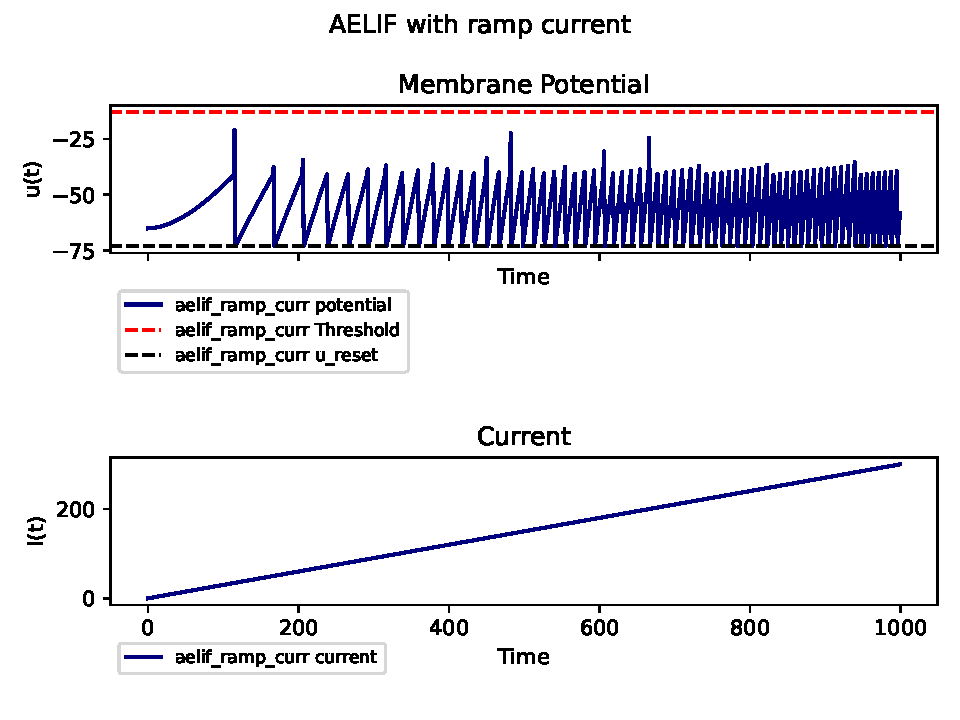
\includegraphics[width=0.8\textwidth]{plots/AELIF with ramp current.pdf} 
                    \caption{مدل تجمیع و آتش نشتی نمایی تطبیق پذیر با جریان شیبدار}
                    \label{fig:aelif-ramp-curr}
                \end{figure}
                همچنین اگر این نمودار را با جریان شیبدار در مدل 
                $ELIF$ 
                مقایسه کنید، متوجه می شود که با اینکه شیب جریان در هر دو یکی است، فرکانس ضربه
                ($spike$) 
                در مدل 
                $AELIF$ 
                دیر تر افزایش می یابد که نشان دهنده تاثیر تطبیق پذیری این مدل است.

            \subsubsection{جریان لگاریتمی}
                آخرین جریان، جریان لگاریتمی است. همانطور که در بخش بالا گفته شد، با اینکه این جریان نیز در مرور زمان افزایش می یابد، ولی در نهایت بعد از مدتی تطبیق پذیری اتفاق می افتد. این مورد از نمودار

                معلوم است.

                \begin{figure}[H]
                    \centering
                    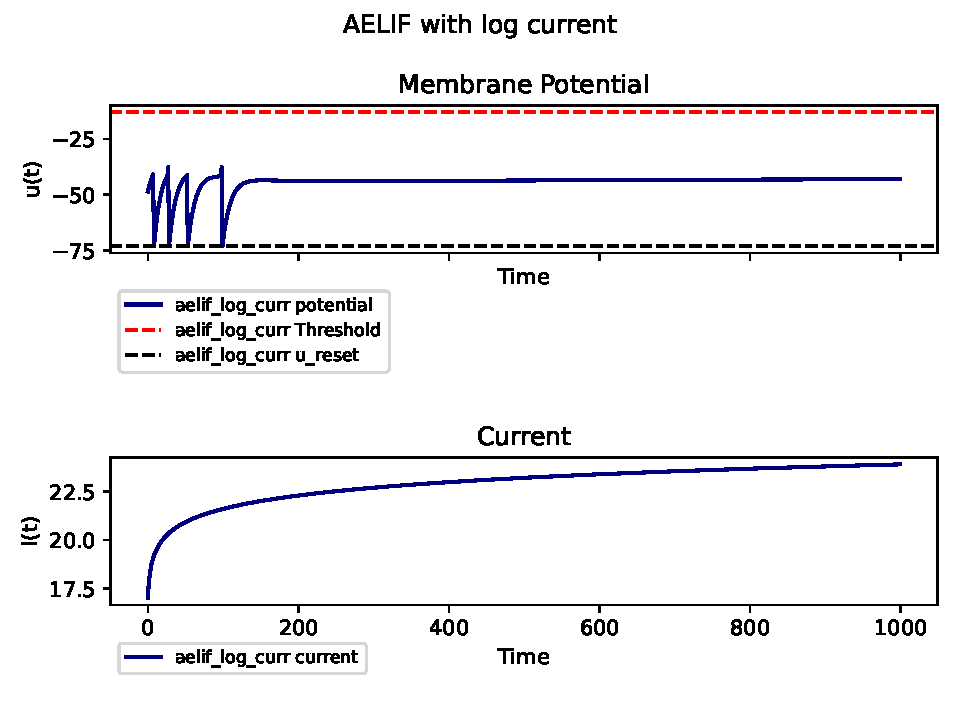
\includegraphics[width=0.8\textwidth]{plots/AELIF with log current.pdf} 
                    \caption{مدل تجمیع و آتش نشتی نمایی تطبیق پذیر با جریان لگاریتمی}
                    \label{fig:aelif-log-curr}
                \end{figure}
                \begin{figure}[H]
                    \centering
                    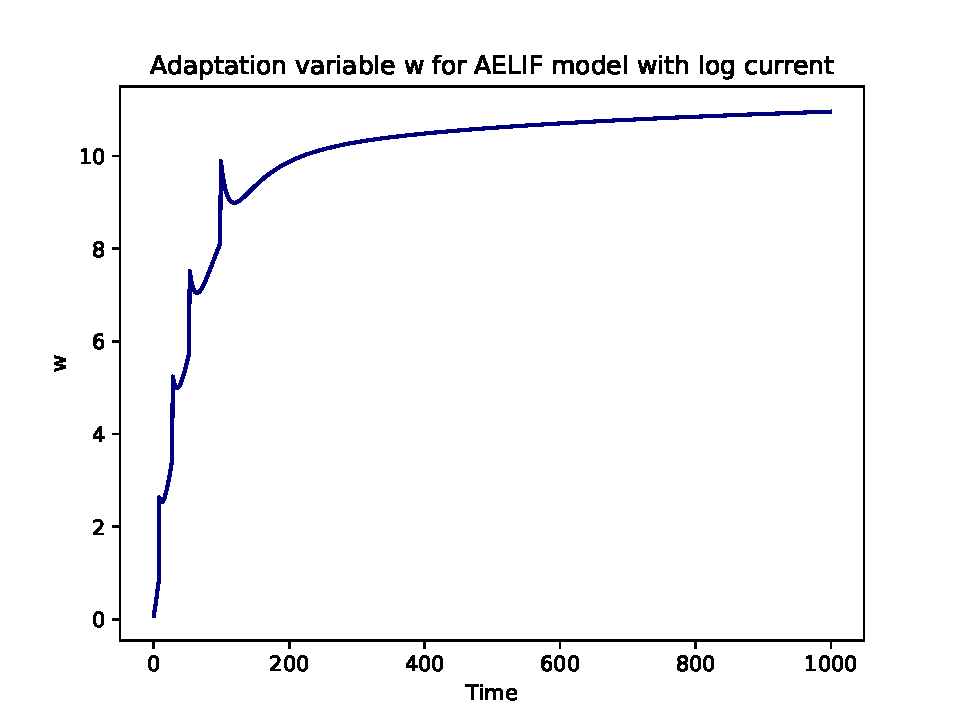
\includegraphics[width=0.8\textwidth]{plots/Adaptation variable w for AELIF model with log current.pdf} 
                    \caption{تغییرات $w$ در مدل تجمیع و آتش نشتی نمایی تطبیق پذیر با جریان لگاریتمی}
                    \label{fig:aelif-w-log-curr}
                \end{figure}
                مجددا، آزمودن پارامتر ها با مقادیر مختلف، تاثیر مشابهی با جریان ثابت خواهد داشت(بعد از مدتی).


\newpage
    \section{افزودن نویز به جریان}
        در این قسمت از پروژه، میخواهیم رفتار نورون هنگام اضافه کردن نویز به جریان را بررسی کنیم. ابتدا از نظر پیاده سازی آن را بررسی میکنیم. برای پیاده سازی نویز، ما به ۲ صورت میتوانیم به این مفهوم نگاه کنیم:
        \begin{itemize}
            \item \textbf{نویز به عنوان یک پارامتر:} در این دیدگاه، نویز در رفتار جریان یا در رفتار مدل نورونی روی جریان اعمال می شود. مثلا هنگام محاسبه جریان در هر یک از این دو، به علاوه یک  ضریبی از یک تابع تصادفی
            (مثلا $uniform$) 
            می شود.
            \item \textbf{نویز به عنوان یک رفتار:} در این دیدگاه، نویز به عنوان یک رفتار دیده می شود. به شخصه این نوع دیدگاه را نسبت به دیدگاه دیگر ترجیه میدهم. در این حالت، یک رفتار نویزی تعریف می شود، و در هر تکرار زمانی، قبل یا بعد از رفتار جریان، روی جریان اعمال می شود.
        \end{itemize}
        لازم به ذکر است که پیاده سازی هر یکی از دیدگاه های بالا، تغییری در نتیجه ایجاد نمیکند، صرفا ممکن است پیاده سازی ما را در آینده پیچیده تر یا ساده تر کند. من هر دو حالت را برای این پروژه پیاده سازی کردم و نتیجه یکسانی گرفتم.
        
        دو نوع نویز سفید و قهوه ای
        (تجمیع نویز سفید)
        در این پروژه در نظر گرفته شده است که هر یک روی توابع جریان اعمال شده و نتیجه نمایش داده شده است. همچنین در نهایت، جریان نویز قهوه ای نیز به عنوان جریان ورودی در نظر گرفته شده است.

        \subsection{مدل نورونی تجمیع و آتش نشتی ساده}
            \subsubsection{جریان ثابت به همراه نویز}
                اولین نمودار
                (شکل \ref{fig:lif-const-noise-curr})
                ، مربوط به جریان ثابت به همراه نویز است. همانطور که مشاهده می شود، افزودن نویز به جریان ثابت، تاثیری در رفتار نورون ندارد و فقط مقدار کمی در نمودار اختلاف پتانسیل نیز نویز ایجاد می کند.
                \begin{figure}[H]
                    \centering
                    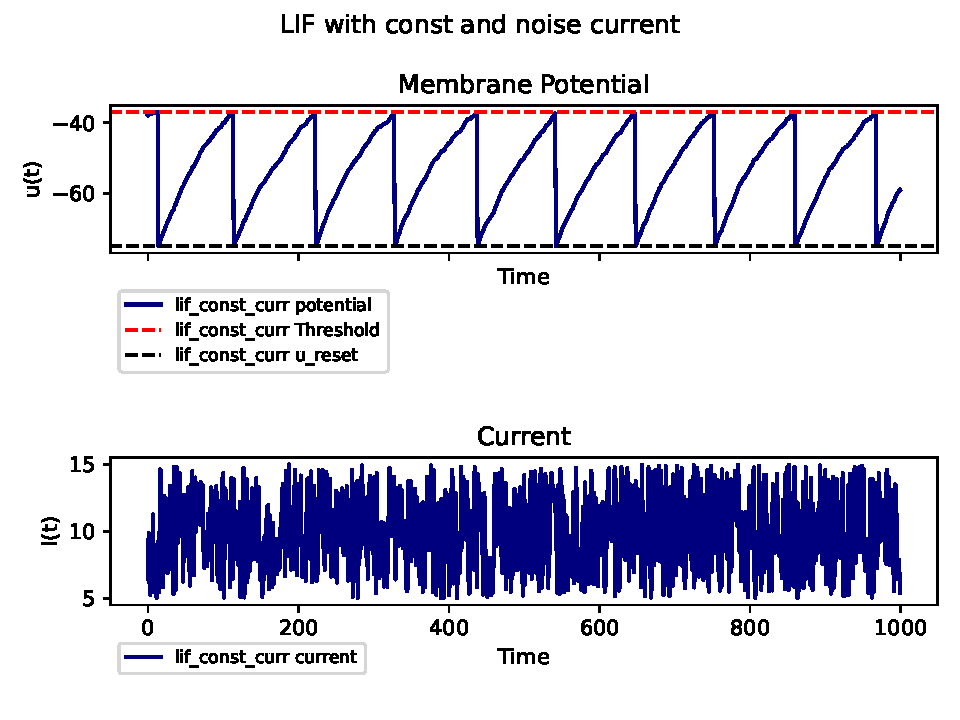
\includegraphics[width=0.8\textwidth]{plots/LIF with const and noise current.pdf} 
                    \caption{مدل تجمیع و آتش نشتی با جریان ثابت نویزدار}
                    \label{fig:lif-const-noise-curr}
                \end{figure}
                واضح است که اگر نویز به صورت با شدت افزایش یابد، فعالیت نورون به کل مختل می شود و دیگر حتی به مدل یا جریان آن وابستگی ندارد.(شکل \ref{fig:lif-const-noise-extreme-curr})
                \begin{figure}[H]
                    \centering
                    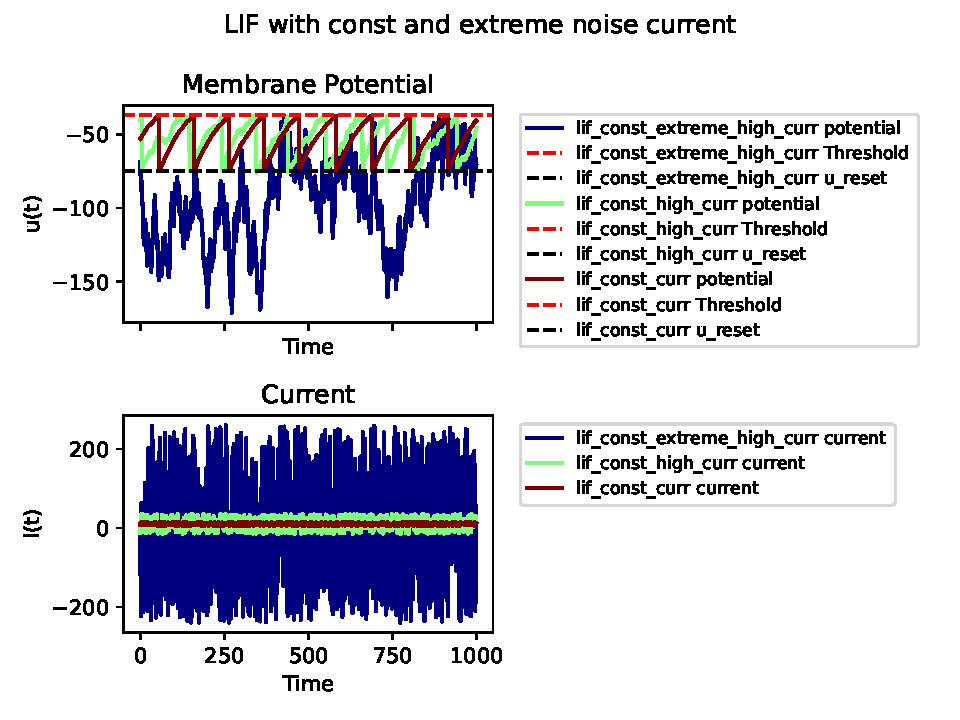
\includegraphics[width=0.8\textwidth]{plots/LIF with const and extreme noise current.pdf} 
                    \caption{مدل تجمیع و آتش نشتی با جریان ثابت نویزدار زیاد}
                    \label{fig:lif-const-noise-extreme-curr}
                \end{figure}
            \subsubsection{جریان پله ای به همراه نویز}
                در این جریان نیز واضح است که انتظار داشته باشیم در بازه ای که جریان وجود دارد همانند جریان ثابت رفتار شود و نمودار
                \ref{fig:lif-step-noise-curr}
                گواه این انتظار است.
                \begin{figure}[H]
                    \centering
                    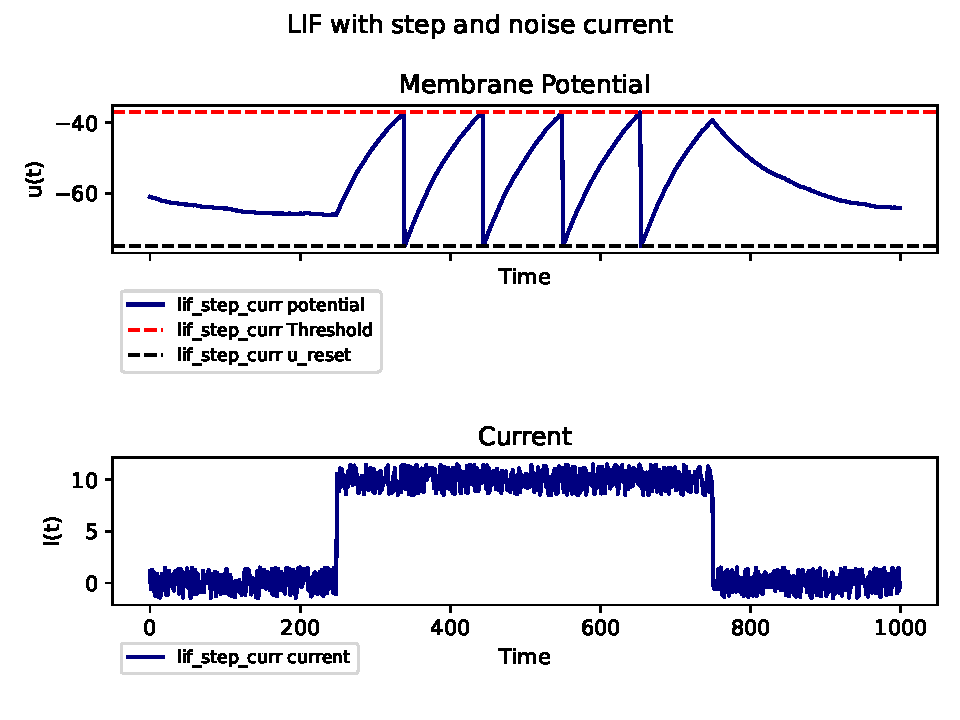
\includegraphics[width=0.8\textwidth]{plots/LIF with step and noise current.pdf} 
                    \caption{مدل تجمیع و آتش نشتی با جریان پله ای نویزدار}
                    \label{fig:lif-step-noise-curr}
                \end{figure}
                تغییرات پارامتر ها در مدل یا نویز، قبل تر توضیح داده شده و ترکیب کردن تغییرات این پارامتر ها، معادل ترکیب کردن اتفاقات بررسی شده تا الان می باشد و نشان دادن نمودار جدید، چیز جدیدی اضافه نمی کند.
            \subsubsection{جریان سینوسی}
                اضافه کردن نویز به جریان سینوسی نیز، تغییری در رفتار نورون اضافه نمی کند و به طور کلی می توان نتیجه گرفت که نورون 
                $LIF$ 
                نسبت به نویز (تا حد معقولی)
                مقاوم است. این موضوع در نمودار 
                \ref{fig:lif-sin-noise-curr}
                معلوم است.
                \begin{figure}[H]
                    \centering
                    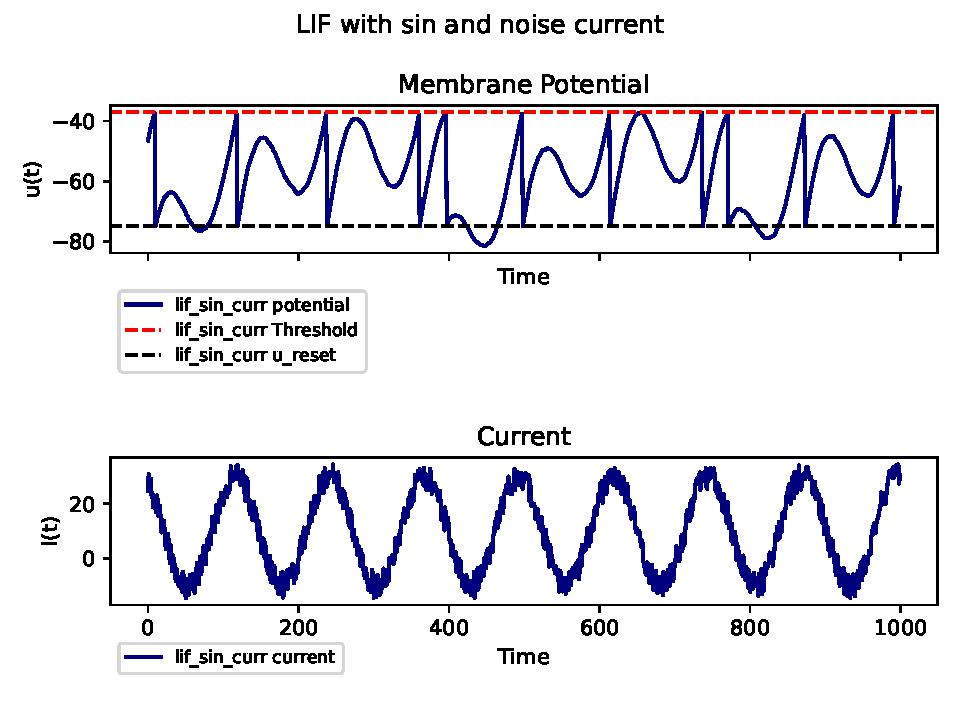
\includegraphics[width=0.8\textwidth]{plots/LIF with sin and noise current.pdf} 
                    \caption{مدل تجمیع و آتش نشتی با جریان سینوسی نویزدار}
                    \label{fig:lif-sin-noise-curr}
                \end{figure}
            \subsubsection{جریان نویز قهوه ای}
                حال اگر یک جریان کاملا نویز دار مانند جریان نویز قهوه ای را به عنوان جریان ورودی به نورون بدهیم چه اتفاقی می افتد؟ این سوال از نمودار 
                \ref{fig:lif-brownian-noise-curr}
                قابل جواب دادن است.
                \begin{figure}[H]
                    \centering
                    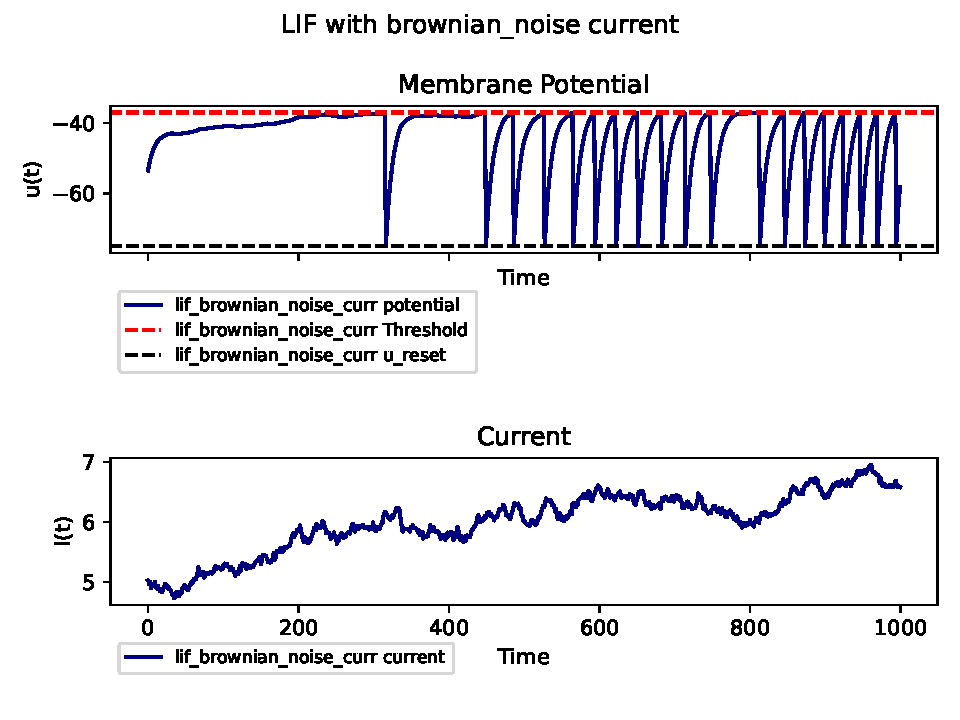
\includegraphics[width=0.8\textwidth]{plots/LIF with brownian_noise current.pdf} 
                    \caption{مدل تجمیع و آتش نشتی با جریان نویز قهوه ای}
                    \label{fig:lif-brownian-noise-curr}
                \end{figure}
                تحلیل خود این نمودار به طور کلی منطقی به نظر نمی رسد، چرا که این جریان برآیند یک سری اعداد تصادفی است. اما این جریان می تواند در فهم توانایی مدل ما کمک کننده باشد. مثلا همانطور که در نمودار پیداست، جاهایی که جریان نمودار کم بوده، نورون به درستی عمل کرده و جایی که جریان زیاد شده است فرکانس ضربه زدن نیز بیشتر شده است.

        \subsection{مدل نورونی تجمیع و آتش نشتی نمایی}
            در این مدل نیز پیش بینی ما این است که افزودن نویز به جریان ها، تفاوتی در رفتار نورون ایجاد نکند.
            \subsubsection{جریان ثابت به همراه نویز}
                همانطور که پیش بینی کردیم، نمودار جریان ثابت به همراه نویز 
                (شکل \ref{fig:lif-const-noise-curr})
                تغییری در رفتار مدل 
                $ELIF$ 
                نسبت به حالت بدون نویز ایجاد نمی کند و فقط نویز های ریزی در نمودار اختلاف پتانسیل مشاهده می شود.
                \begin{figure}[H]
                    \centering
                    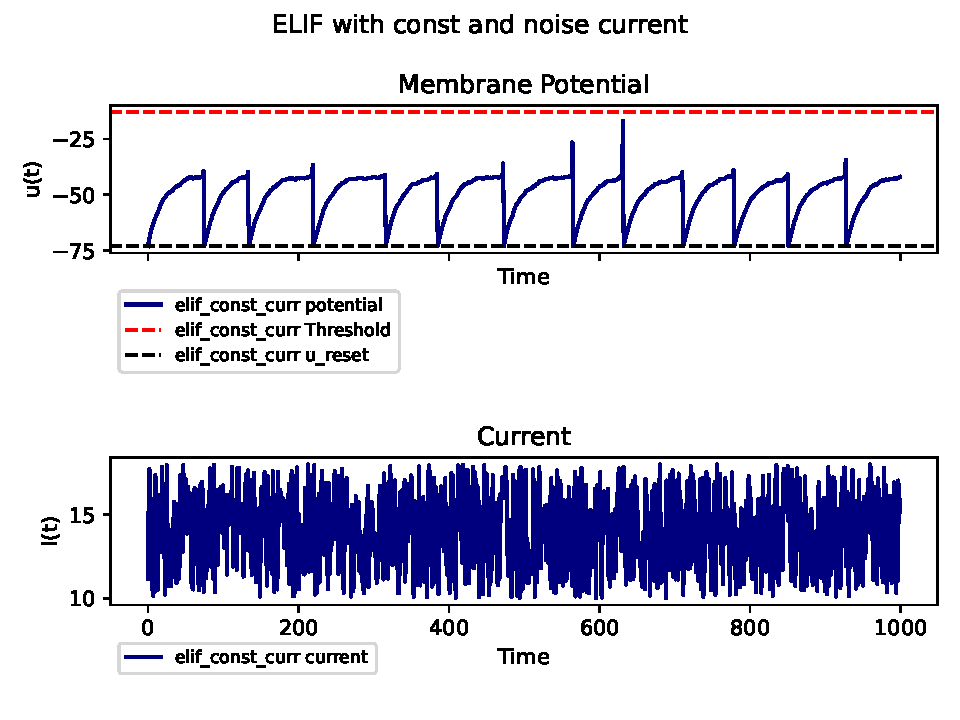
\includegraphics[width=0.8\textwidth]{plots/ELIF with const and noise current.pdf} 
                    \caption{مدل تجمیع و آتش نشتی نمایی با جریان ثابت نویزدار  }
                    \label{fig:elif-const-noise-curr}
                \end{figure}

            \subsubsection{جریان پله ای به همراه نویز}
                تاثیر نویز بر این جریان بعد از زمان
                $t_1$ 
                نیز همانند تاثیر نویز بر جریان ثابت است.
                (شکل \ref{fig:elif-step-noise-curr})

                \begin{figure}[H]
                    \centering
                    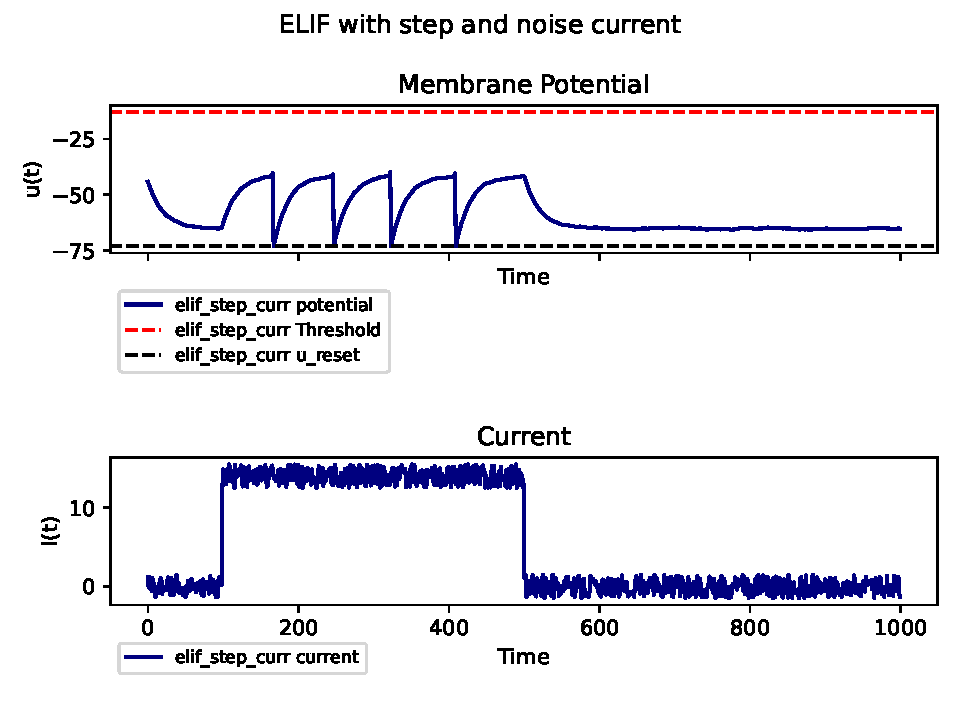
\includegraphics[width=0.8\textwidth]{plots/ELIF with step and noise current.pdf} 
                    \caption{مدل تجمیع و آتش نشتی نمایی با جریان پله ای نویزدار  }
                    \label{fig:elif-step-noise-curr}
                \end{figure}
            \subsubsection{جریان سینوسی به همراه نویز}
                جریان سینوسی نیز در صورت اضافه شدن نویز به آن تاثیر خاصی روی عملکرد نورون نمیگذارد و رفتار نورون با جریان سینوسی نیز نسبت به نویز مقاوم است.
                (شکل \ref{fig:elif-sin-noise-curr})
                \begin{figure}[H]
                    \centering
                    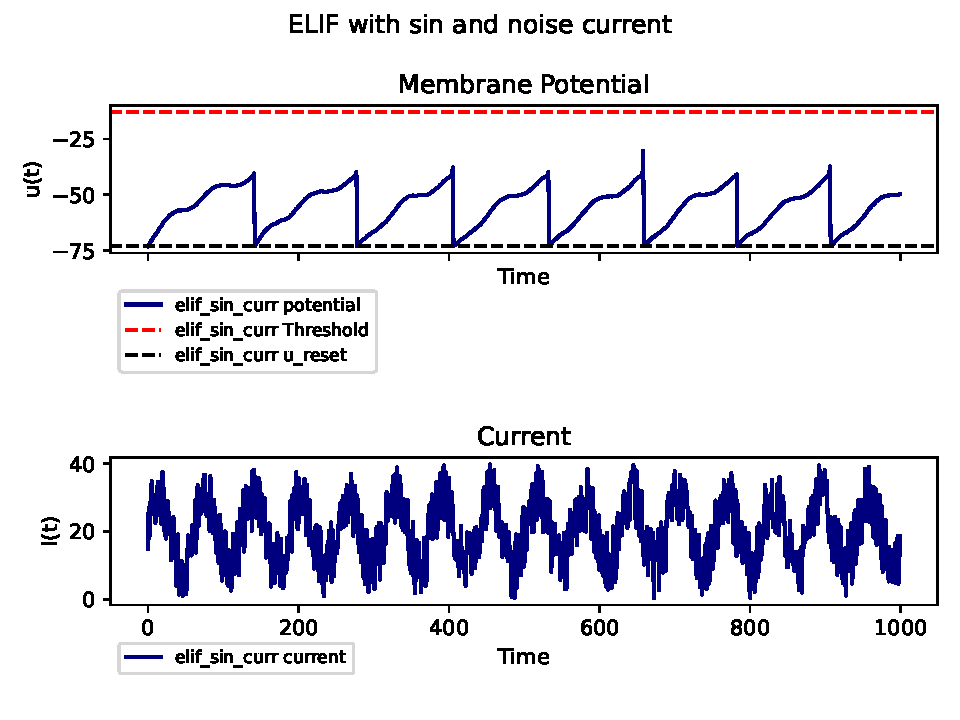
\includegraphics[width=0.8\textwidth]{plots/ELIF with sin and noise current.pdf} 
                    \caption{مدل تجمیع و آتش نشتی نمایی با جریان سینوسی  نویزدار  }
                    \label{fig:elif-sin-noise-curr}
                \end{figure}

            \subsubsection{جریان نویز قهوه ای}
                همانطور که در ابتدای این بخش گفتیم، حتی جریان کاملا تصادفی قهوه ای نیز تاثیری بر روی رفتار نورون در این مدل ندارد و اگر این مدل را با مدل ساده 
                $LIF$ 
                مقایسه کنید، متوجه می شوید که تنها در بالا رفتن اختلاف پتانسیل غشا بعد از پتانسیل 
                $u_{rh}$ 
                تفاوت دارند.
                (شکل \ref{fig:elif-brownian-noise-curr})
                \begin{figure}[H]
                    \centering
                    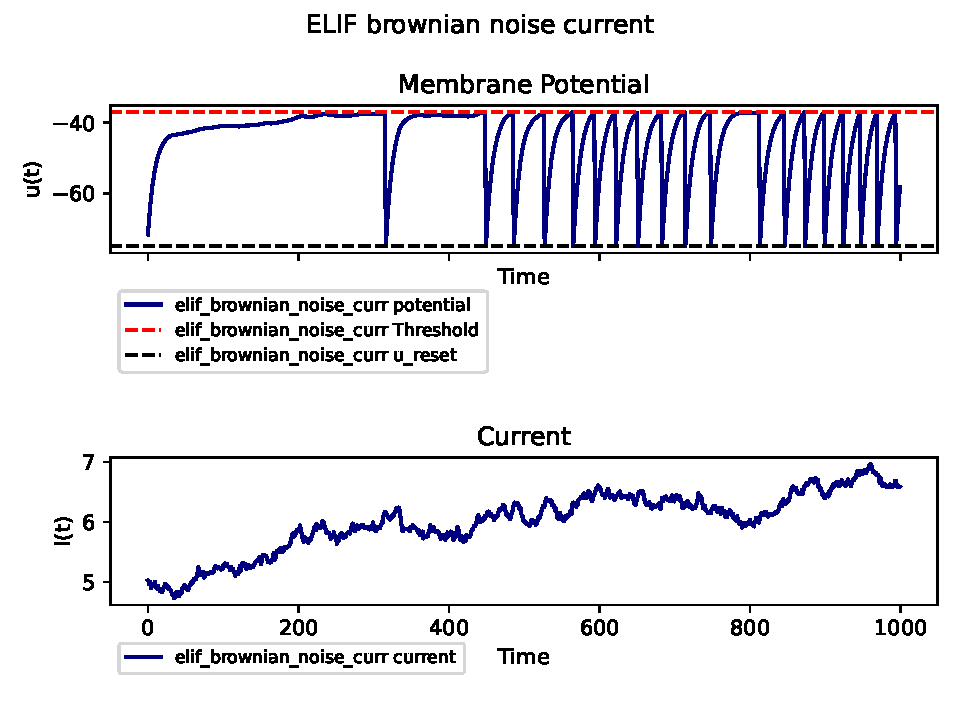
\includegraphics[width=0.8\textwidth]{plots/ELIF brownian noise current.pdf} 
                    \caption{مدل تجمیع و آتش نشتی نمایی با جریان نویز قهوه ای  }
                    \label{fig:elif-brownian-noise-curr}
                \end{figure}
        \subsection{مدل نورونی تجمیع و آتش نشتی نمایی تطبیق پذیر}
            عملکرد مدل نورونی تجمیع و آتش نشتی نمایی تطبیق پذیر نیز با افزودن نویز تغییری نخواهد کرد. تنها حالتی که نسبت به حالت های قبلی می تواند جالب باشد، حالت جریان نویز قهوه ای است که در ادامه آن را بررسی میکنیم.
            \subsubsection{جریان ثابت نویزدار} 
                همانطور که مشاهده می شود، افزودن نویز به جریان ثابت تغییری در رفتار تطبیق پذیری مدل ما ایجاد نمی کند.                
                (شکل \ref{fig:aelif-const-noise-curr})   
                \begin{figure}[H]
                    \centering
                    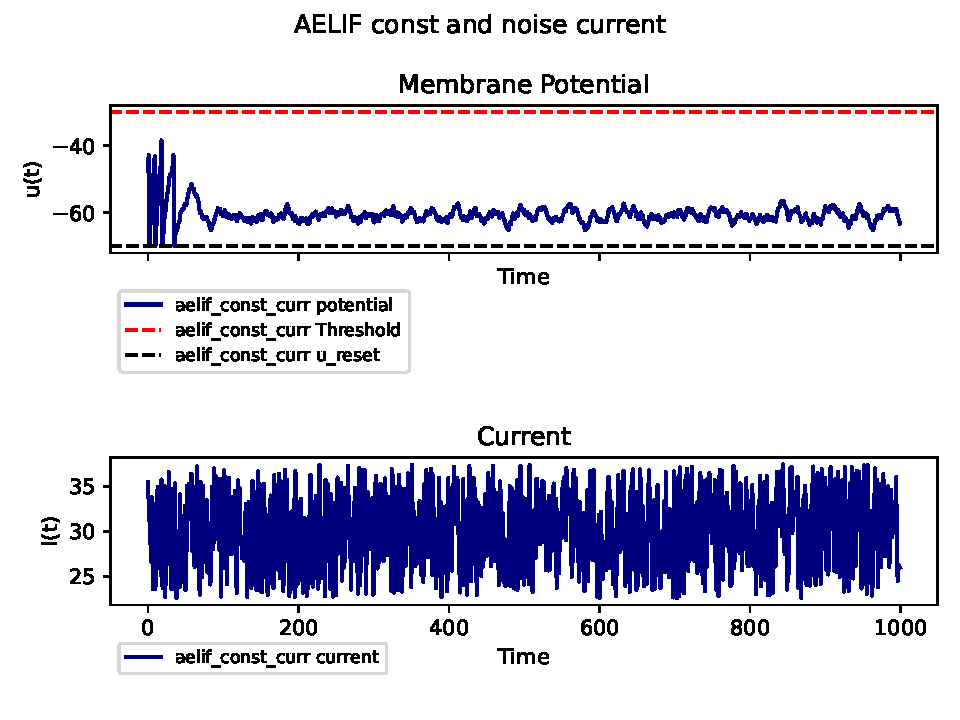
\includegraphics[width=0.8\textwidth]{plots/AELIF const and noise current.pdf} 
                    \caption{مدل تجمیع و آتش نشتی نمایی تطبیق پذیر با جریان ثابت نویزدار  }
                    \label{fig:aelif-const-noise-curr}
                \end{figure}
                نکته جالب در این نمودار این است که مدل 
                $AELIF$ 
                نسبت به نویز تطبیق نمی یابد و خود نویز ها در نمودار اختلاف پتانسیل نیز قابل مشاهده هستند و فقط ضربه
                ($spike$) 
                زده نمی شود.

            \subsubsection{جریان پله ای نویزدار}
                برای جریان پله ای نیز مانند گذشته، انتظار داریم که از لحظه 
                $t_1$ 
                به بعد مانند جریان ثابت رفتار کند. نمودار 
                \ref{fig:aelif-step-noise-curr} 
                نیز ادعای ما را تایید می کند.
                \begin{figure}[H]
                    \centering
                    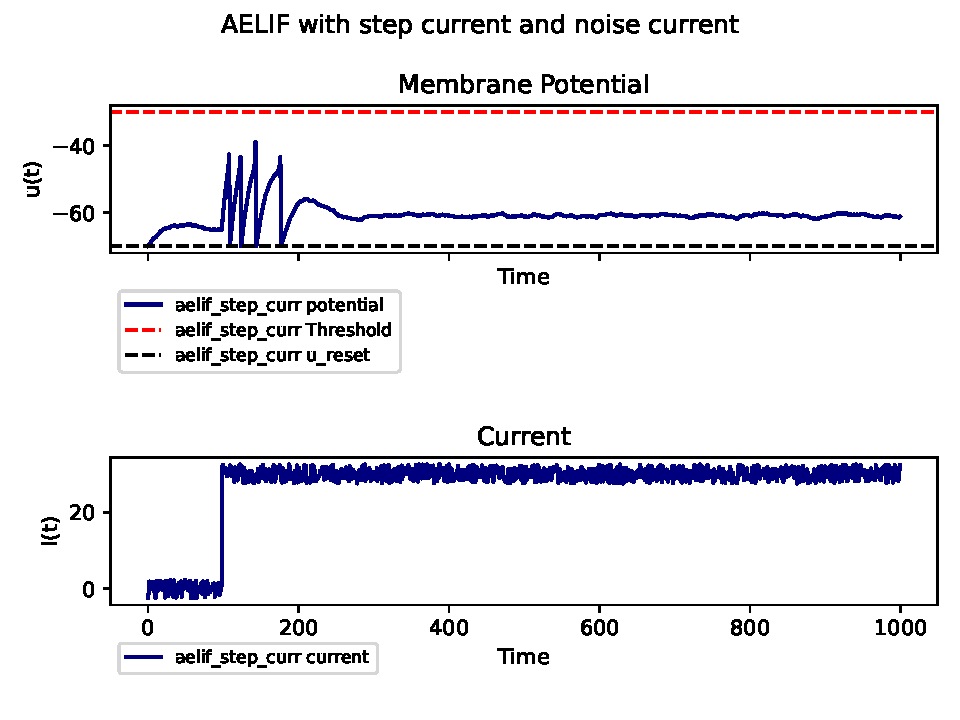
\includegraphics[width=0.8\textwidth]{plots/AELIF with step current and noise current.pdf} 
                    \caption{مدل تجمیع و آتش نشتی نمایی تطبیق پذیر با جریان پله ای نویزدار  }
                    \label{fig:aelif-step-noise-curr}
                \end{figure}
            \subsubsection{جریان سینوسی نویزدار}
                در حالت بدون نویز مشاهده کردیم که در جریان سینوسی تطبیق پذیری آهسته تر اتفاق می افتد. این رفتار نیز در جریان نویزدار تکرار شده و تغییری رخ نمی دهد.
                (شکل \ref{fig:aelif-sin-noise-curr})
                \begin{figure}[H]
                    \centering
                    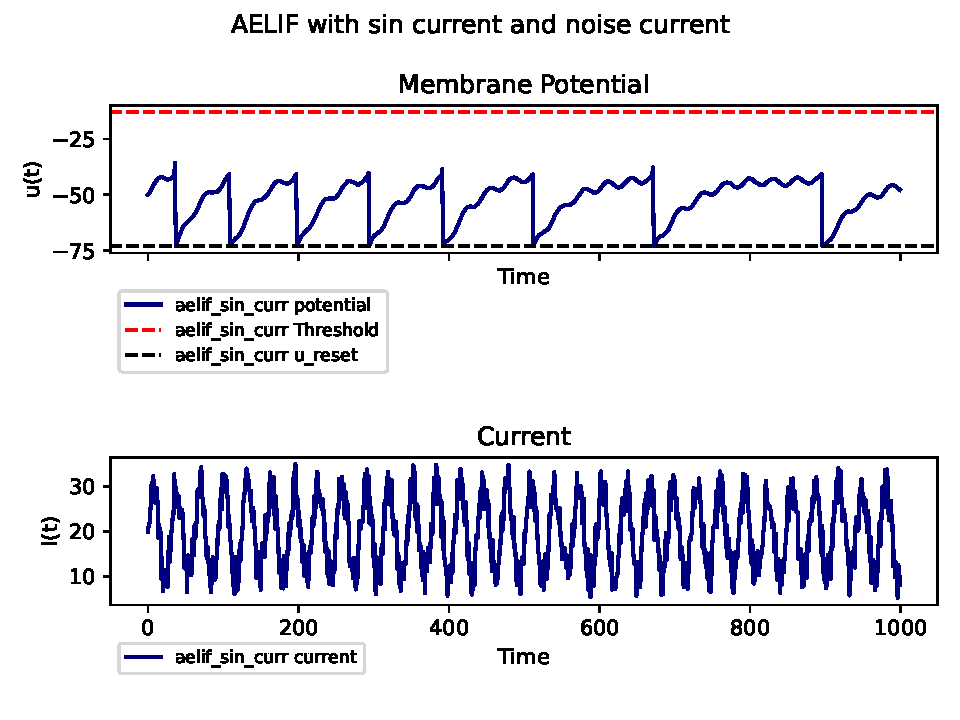
\includegraphics[width=0.8\textwidth]{plots/AELIF with sin current and noise current.pdf} 
                    \caption{مدل تجمیع و آتش نشتی نمایی تطبیق پذیر با جریان سینوسی نویزدار  }
                    \label{fig:aelif-sin-noise-curr}
                \end{figure}
            \subsubsection{جریان نویز قهوه ای}
                به نظر من تنها مورد جالب برای بررسی در این بخش، همین جریان کاملا تصادفی می باشد. چرا که همانطور که از شکل
                \ref{fig:aelif-brownian-noise-curr} و 
                \ref{fig:aelif-w-brownian-noise-curr}
                دریافت می شود، مدل نسبت به حالت های قبلی خیلی دیرتر تطبیق می یابد، ضمن اینکه بعد از تطبیق یافتن حتی با افزایش جریان، دیگر ضربه ای در نورون زده نمی شود که نشان دهنده تطبیق رخ داده در نورون است.
                \begin{figure}[H]
                    \centering
                    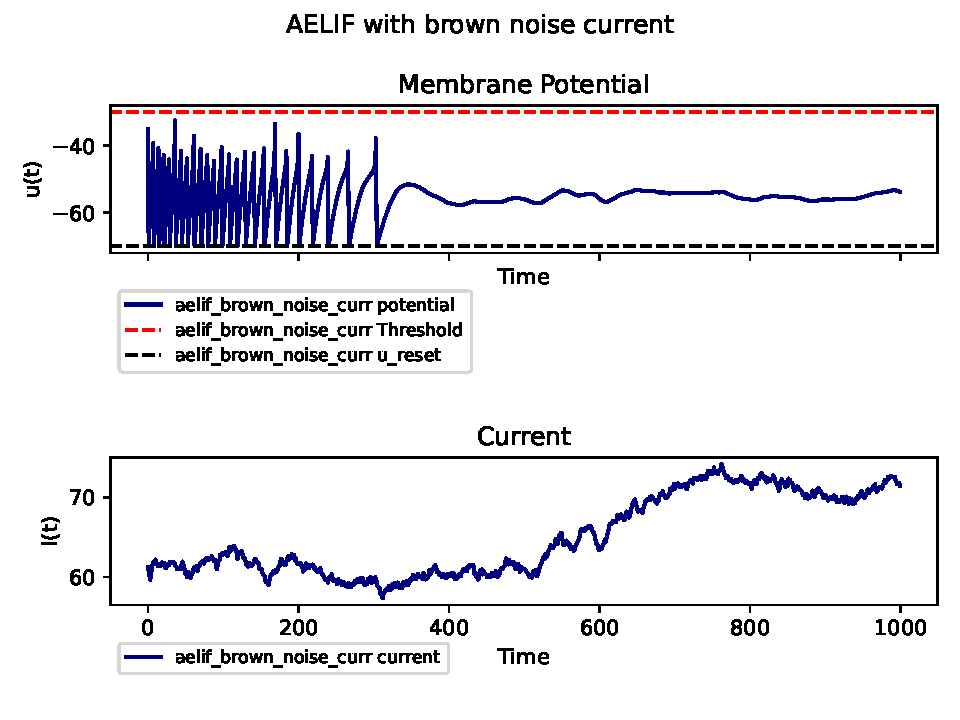
\includegraphics[width=0.8\textwidth]{plots/AELIF with brown noise current.pdf} 
                    \caption{مدل تجمیع و آتش نشتی نمایی تطبیق پذیر با جریان نویز قهوه ای  }
                    \label{fig:aelif-brownian-noise-curr}
                \end{figure}
                \begin{figure}[H]
                    \centering
                    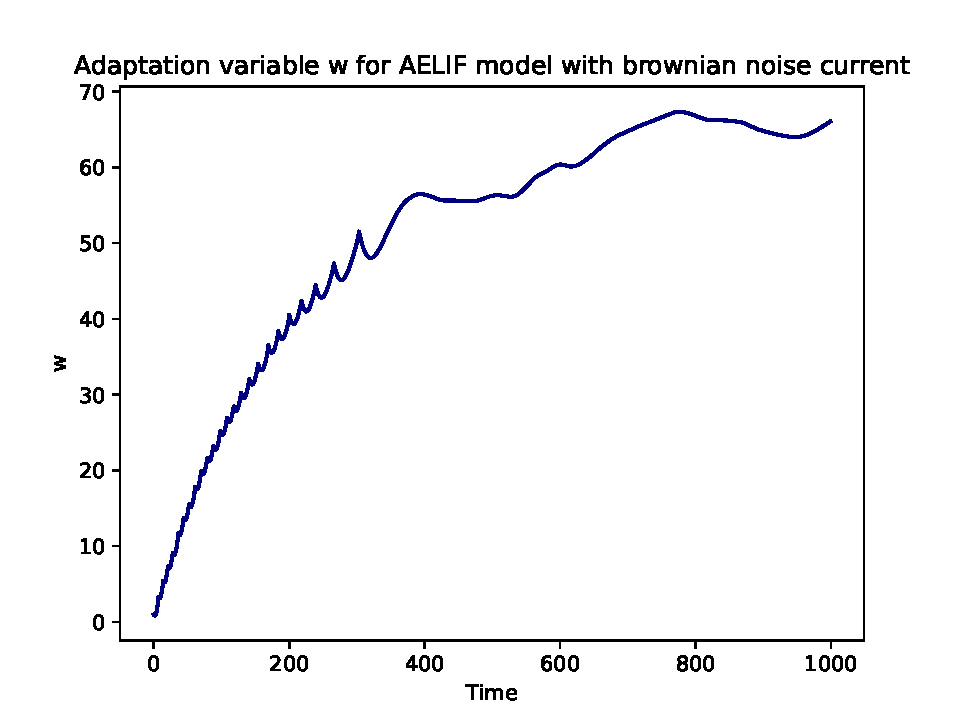
\includegraphics[width=0.8\textwidth]{plots/Adaptation variable w for AELIF model with brownian noise current.pdf} 
                    \caption{تغییرات $w$ در مدل تجمیع و آتش نشتی نمایی تطبیق پذیر با جریان نویز قهوه ای}
                    \label{fig:aelif-w-brownian-noise-curr}
                \end{figure}
\newpage
    \section{نمودار منحنی $I-F$}
        در این بخش میخواهیم مدل هایمان را با استفاده از ۲۰ جریان مختلف از  تا ۲۰ با دو نوع جریان ثابت و جریان ثابت نویز دار آزمایش کنیم، و تغییرات فرکانس ضربه
        ($spike$) 
        را در آن ها مقایسه کنیم. به طور کلی انتظار داریم که طبق نمودار های قبلی ، هردو منحنی بدون نویز و نویز دار بر یک دیگر منطبق باشند.
        منحنی 
        $I-F$ 
        که به عنوان منحنی جریان-فرکانس نیز شناخته می شود، یک نمایش گرافیکی است که معمولاً برای توصیف رابطه بین جریان ورودی 
        ($I$) 
        به یک نورون و فرکانس ضربه حاصله 
        ($F$)
        پتانسیل های عمل ایجاد شده توسط آن استفاده می شود. به طور معمول، با افزایش جریان ورودی، فرکانس ضربه نیز افزایش می یابد. 
        
        \subsection{مدل تجمیع و آتش نشتی ($LIF$)}
            همانطور که در بخش قبلی دیدیم، انتظار داریم که اضافه کردن نویز به جریان، رفتار نورون ها را تغییر نداده و در نتیجه، فرکانس ضربه زدن نیز با نویز تغییر نکند. نمودار 
            \ref{fig:lif-noise-curr-I-F}
            می تواند فرضیه ما را تقویت کند.
            \begin{figure}[H]
                \centering
                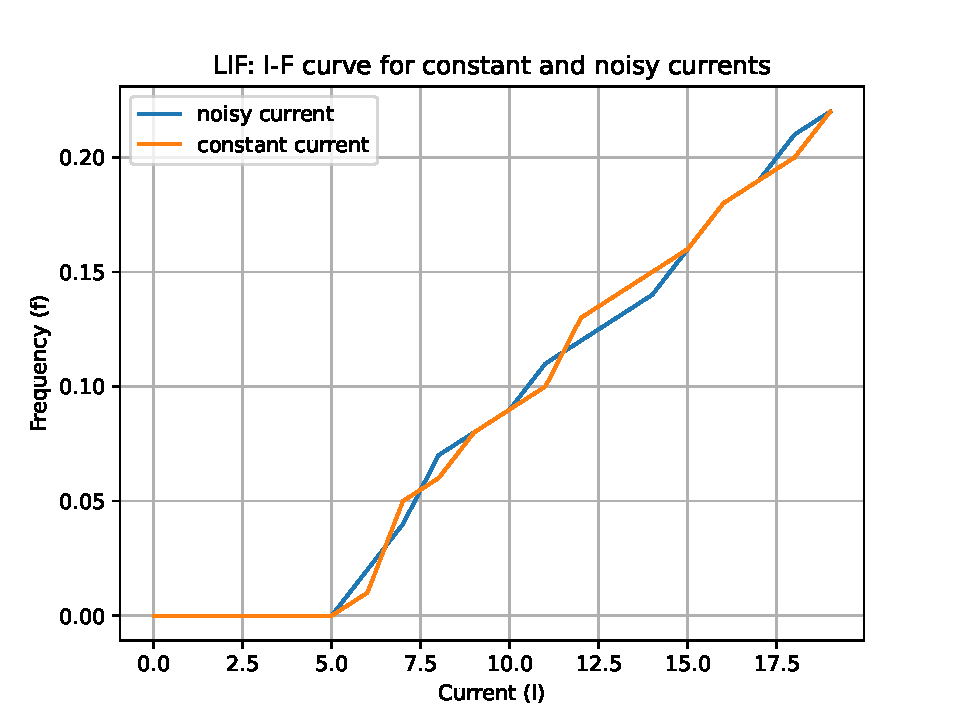
\includegraphics[width=0.8\textwidth]{plots/LIF: I-F curve for constant and noisy currents.pdf} 
                \caption{نمودار $I-F$ برای مدل تجمیع و آتش نشتی  }
                \label{fig:lif-noise-curr-I-F}
            \end{figure}
            همانطور که ملاحظه می شود، افزودن نویز چه در جریان کم چه در جریان زیاد، رفتار نورون $LIF$ را تغییر نمی دهد.
        \subsection{مدل تجمیع و آتش نشتی نمایی ($ELIF$)}
            به طور مشابه از بخش قبل انتظار داریم که اضافه کردن نویز به جریان، رفتار نورون ها را تغییر نداده و در نتیجه، فرکانس ضربه زدن نیز با نویز تغییر نکند. از نمودار
            \ref{fig:elif-noise-curr-I-F}
            دریافت می شود که این ادعا برای جریان های زیاد می تواند درست باشد، اما درمورد جریان های کم با قاطعیت نمیتوان صحبت کرد. حدس من این است که در جریان های کم، یک نویز می تواند اختلاف پتانسیل نورون را به 
            $u_{rh}$ 
            نزدیک کند در حالی که در جریان های بالا، این نویز تاثیرش کمتر می شود.(چرا که مثلا اگر اختلاف پتانسیل نزدیک 
            $u_{rh}$ 
            باشد، چه نویز زده شود چه زده نشود، احتمالا در لحظه بعدی اختلاف پتانسیل نورون به این آستانه میرسد.)
            هر چند در کل این تفاوت ناچیز و قابل چشم پوشی است و نباید زیاد برای آن حساس شد. 
            \begin{figure}[H]
                \centering
                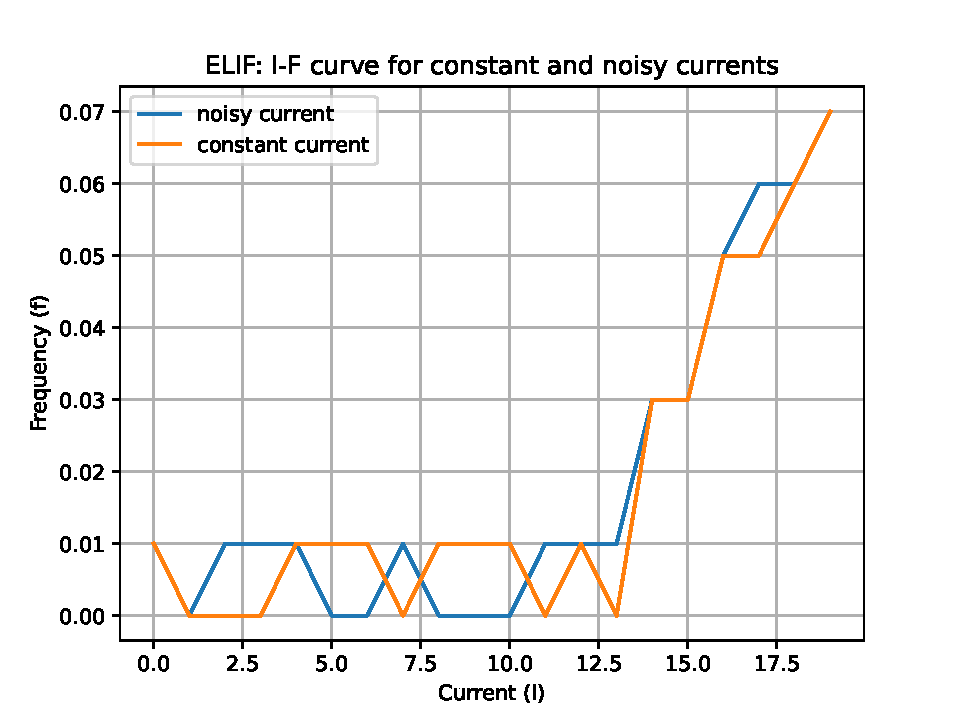
\includegraphics[width=0.8\textwidth]{plots/ELIF: I-F curve for constant and noisy currents.pdf} 
                \caption{نمودار $I-F$ برای مدل تجمیع و آتش نشتی نمایی  }
                \label{fig:elif-noise-curr-I-F}
            \end{figure}
            \subsection{مدل تجمیع و آتش نشتی نمایی تطبیق پذیر ($AELIF$)}
                در این مدل نیز انتظار داریم تفاوت مانند دو مدل دیگر باشد، چرا که این مدل نیز در جریان ثابت نسبت به نویز مقاوم است. نمودار 

                ادعای مارا تثبیت می کند.
                \begin{figure}[H]
                    \centering
                    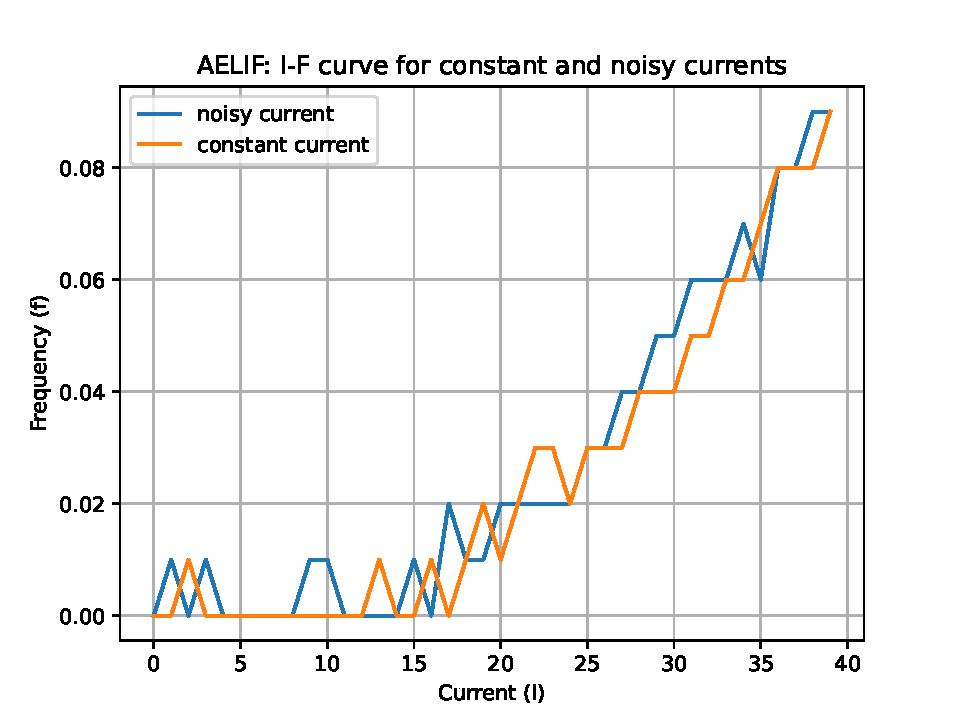
\includegraphics[width=0.8\textwidth]{plots/AELIF: I-F curve for constant and noisy currents.pdf} 
                    \caption{نمودار $I-F$ برای مدل تجمیع و آتش نشتی نمایی تطبیق پذیر  }
                    \label{fig:aelif-noise-curr-I-F}
                \end{figure}
            % Start a new section   
\newpage
    \section{بازه مقاومت}
        بازه مقاومت به مرحله موقتی پس از ضربه
        $spike$ 
        یک نورون گفته می شود که در طی آن نورون در برابر ایجاد پتانسیل عمل دیگری مقاوم است. این دوره برای تنظیم زمان و فرکانس سیگنال دهی عصبی بسیار مهم است. دو نوع اصلی بازه مقاومت وجود دارد: بازه مقاومت مطلق، که در طی آن هیچ مقداری از جریان نمی تواند پتانسیل عمل دیگری را تحریک کند، و بازه مقاومت نسبی، که در طی آن یک محرک قوی تر از حد معمول ممکن است پاسخی را برانگیزد. این بازه ها تضمین می‌کنند که سیگنال‌های عصبی منظم باقی می‌مانند، از شلیک بیش از حد جلوگیری می‌کنند و امکان پردازش دقیق اطلاعات در سیستم عصبی را فراهم می‌کنند.

        \begin{itemize}
            \item دلیل زیست شناسی: بازه مطلق مقاومتی تقریباً کل مدت زمان پتانسیل عمل است، به علت غیرفعال شدن کانال‌های سدیمی است که معمولاً برای دپلاریزاسیون غشا باز می‌شوند که این کانال‌ها تا موقع هایپر پلاریزاسیون غیرفعال می‌مانند سپس کانال‌ها بسته می‌شوند و دوباره توانایی پاسخ به تحریک را پیدا می‌کنند.\cite{wikipedia-refractory-period}
        \end{itemize}
        برای پیاده سازی بازه مقاومت، میتوان دو روش را در نظر گرفت. یک روش، دیدگاه پارامتری دارد، بدین معنا که مدل ها، یک پارامتر 
        \texttt{refractory\_T} 
        را دریافت کرده و براساس آن فرایند بازه مقاومت اعمال می شود، و دیدگاه دیگر، به بازه مقاومت به شکل یک رفتار نگاه می کند و آن را در هر لحظه زمانی، بعد از رفتار جریان، روی نورون اعمال می کند. از نظر پیاده سازی حالت دوم بهتر و تمیز تر به نظر می رسد، اما با توجه به توضیحات بیولوژیکی ارائه شده در بالا، دیدگاه اول به زیست شناسی نزدیک تر است چرا که جریان قطع نمی شود. هر چند من هر دو حالت را پیاده سازی کردم و رفتار نورون ها یکسان بود.

        \subsection{مدل تجمیع و آتش نشتی ($LIF$)}
            در مدل اول، یعنی 
            $LIF$، 
            بازه مقاومت را شبیه سازی میکنیم و سپس براساس نمودار آن را تحلیل میکنیم. فقط برای مدل اول، من نحوه پیاده سازی  به صورت دیدگاه رفتاری را نیز می آورم، اما به آن به صورت یک رفرنس نگاه کرده نمی شود. همچنین از آنجا که رفتار جریان پله ای حدودا مشابه رفتار جریان ثابت می باشد، فقط دو جریان ثابت و سینوسی را بررسی میکنیم.
            \subsubsection{جریان ثابت}
                همانطور که از شکل 
                \ref{fig:lif-const-curr-refractory}
                بر می آید، نورون دارای بازه مقاومت، بعد از هر ضربه
                ($spike$) 
                تا مدتی هیچ ضربه ای نمی زند. همچنین بعد از اینکه بازه مقاومت آن تمام می شود، دیگر با نورون بدون بازه مقاومت در لحظه های یکسان ضربه نمی زند.
                \begin{figure}[H]
                    \centering
                    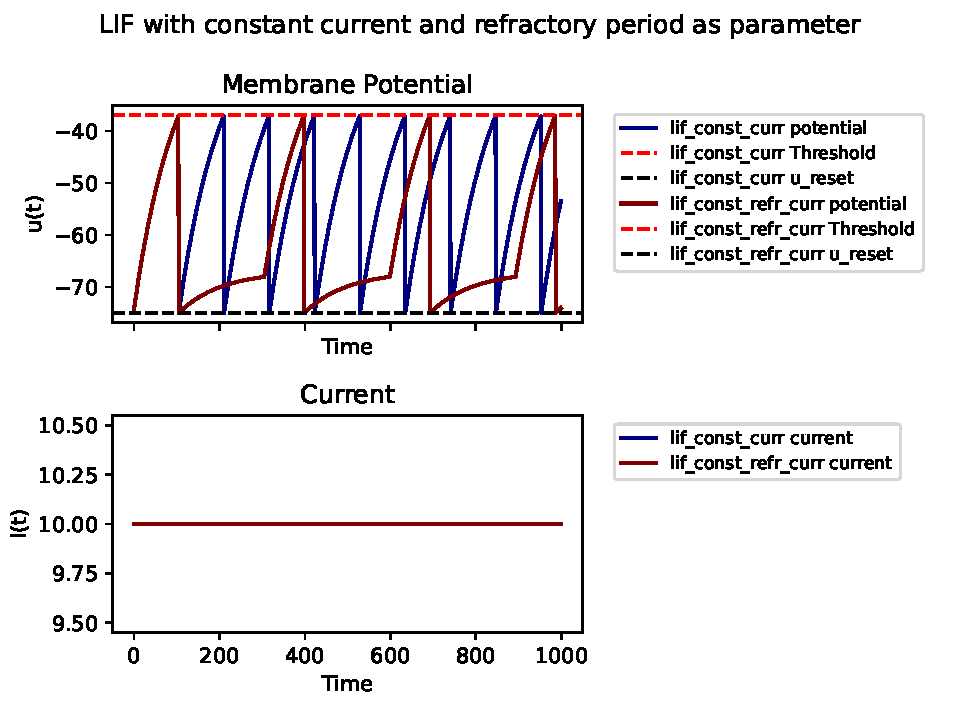
\includegraphics[width=0.8\textwidth]{plots/LIF with constant current and refractory period as parameter.pdf} 
                    \caption{مقایسه لحظات ضربه زدن در مدل $LIF$ ساده با جریان ثابت و با بازه مقاومت}
                    \label{fig:lif-const-curr-refractory}
                \end{figure}
                \begin{figure}[H]
                    \centering
                    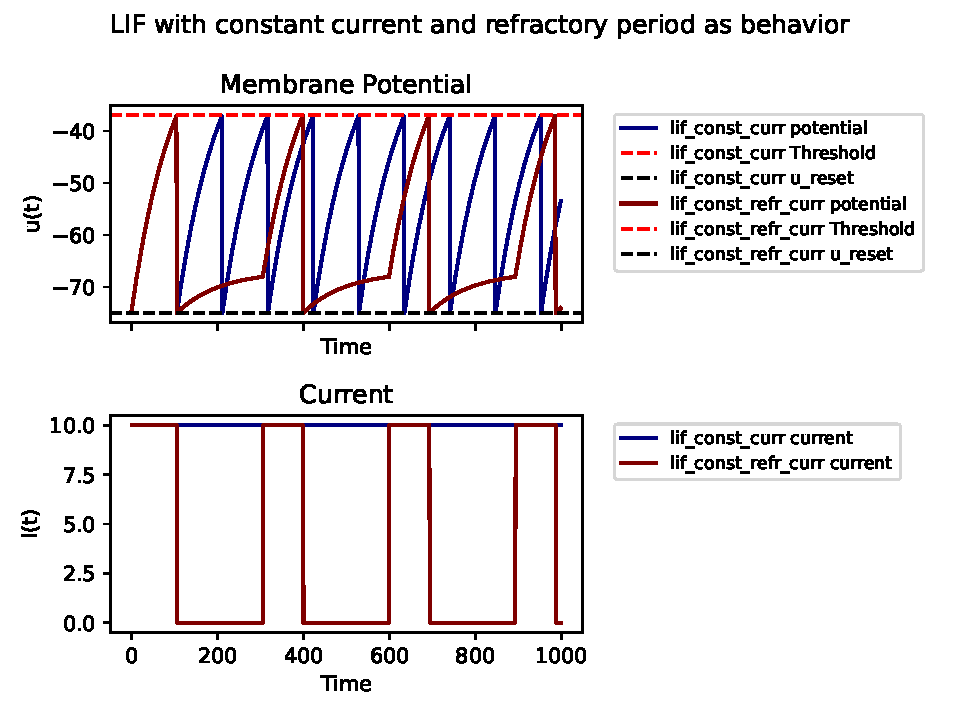
\includegraphics[width=0.8\textwidth]{plots/LIF with constant current and refractory period as behavior.pdf} 
                    \caption{مقایسه لحظات ضربه زدن در مدل $LIF$ ساده با جریان ثابت و با بازه مقاومت با پیاده سازی رفتاری}
                \end{figure}
            \subsubsection{جریان سینوسی}
                در جریان سینوسی نیز اتفاقی مشابه جریان ثابت می افتد و نورون با بازه مقاومت، بعد از هر ضربه، تا لحظاتی جریانی دریافت نمی کند.
                \begin{figure}[H]
                    \centering
                    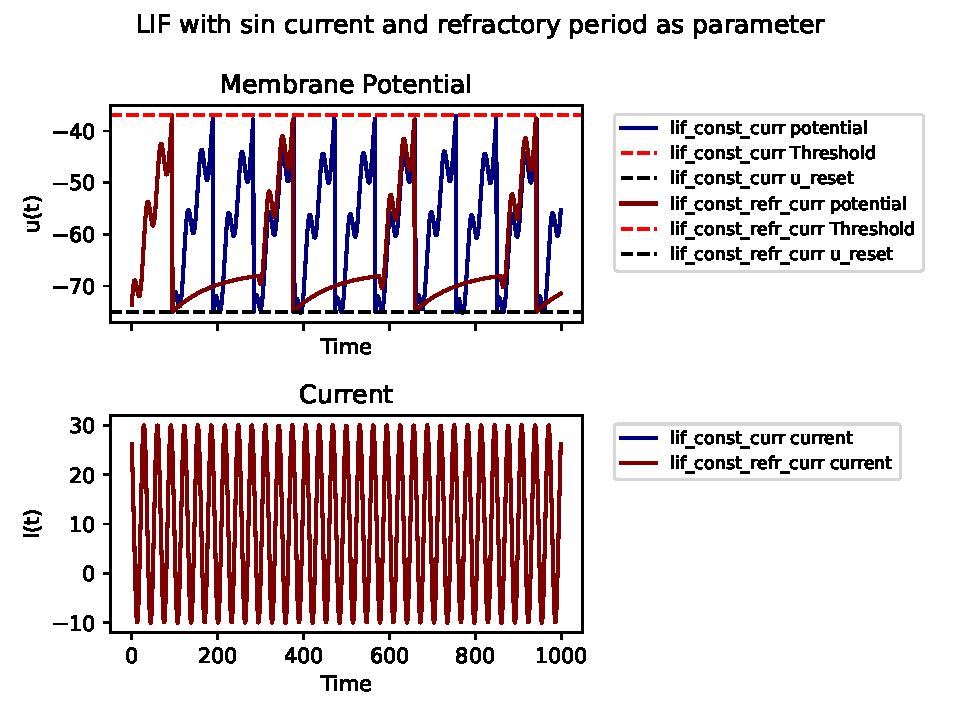
\includegraphics[width=0.8\textwidth]{plots/LIF with sin current and refractory period as parameter.pdf} 
                    \caption{مقایسه لحظات ضربه زدن در مدل $LIF$ ساده با جریان سینوسی و با بازه مقاومت}
                    \label{fig:lif-sin-curr-refractory}
                \end{figure}
        \subsection{مدل تجمیع و آتش نشتی نمایی ($ELIF$)}
            از آنجا که در این بخش آوردن جریان های متفاوت تاثیری در تحلیل بازه مقاومت ندارد، به همان جریان ثابت بسنده می کنیم.
            \begin{figure}[H]
                \centering
                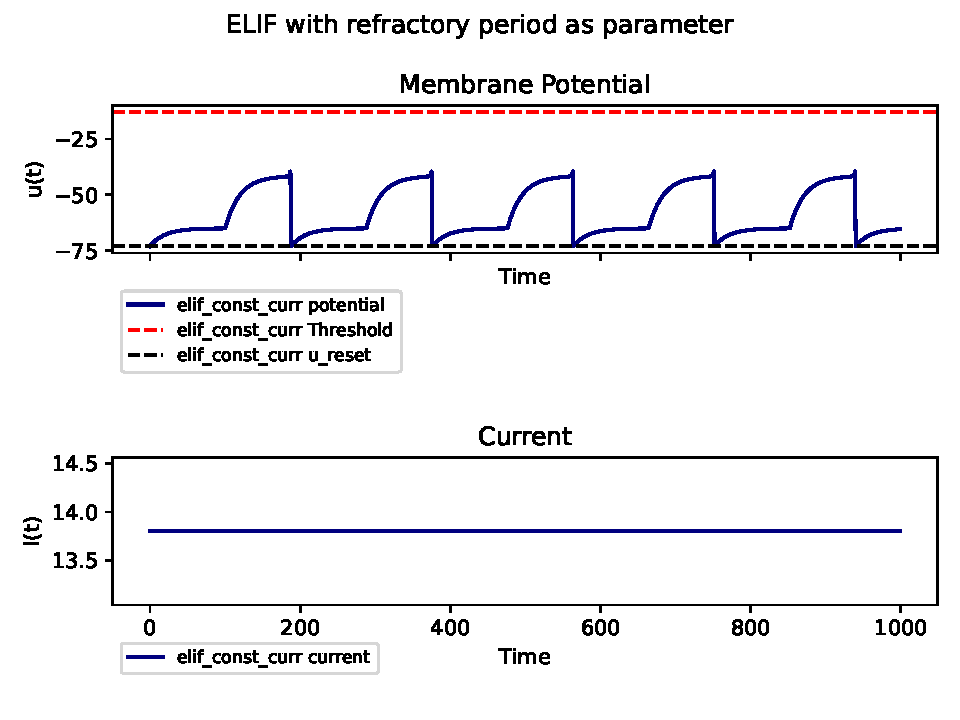
\includegraphics[width=0.8\textwidth]{plots/ELIF with refractory period as parameter.pdf} 
                \caption{مقایسه لحظات ضربه زدن در مدل $ELIF$ ساده با جریان ثابت و با بازه مقاومت}
            \end{figure}
        \subsection{مدل تجمیع و آتش نشتی نمایی تطبیق پذیر ($AELIF$)}
            تنها موردی که به نظر می رسد از نظر تحلیل جذاب باشد، مدل 
            $AELIF$ 
            می باشد. چرا که همانطور که از نمودار 
            \ref{fig:aelif-const-curr-refractory}
            مشخص است، بازه مقاومت زیاد باعث می شود تا تطبیق پذیری نورون از بین برود و برخلاف چیزی که تا الان در مدل 
            $AELIF$ 
            با جریان های ثابت داشتیم، دیگر تطبیق پذیری در آن رخ ندهد. 
            \begin{figure}[H]
                \centering
                \includegraphics[width=0.7\textwidth]{plots/AELIF with refractory period as parameter.pdf} 
                \caption{مقایسه لحظات ضربه زدن در مدل $AELIF$ ساده با جریان ثابت و با بازه مقاومت}
                \label{fig:aelif-const-curr-refractory}
            \end{figure}
            هرچند همانطور که در نمودار 
            \ref{fig:aelif-const-curr-refractory-low}
            دیده می شود، انتخاب بازه مقاومت کم، نمیتواند تاثیر تطبیق پذیری را کم کند و درنتیجه رفتار نورون مشابه حالت عادی می شود و تطبیق می یابد.
            \begin{figure}[H]
                \centering
                \includegraphics[width=0.7\textwidth]{plots/AELIF with refractory period as parameter and low value.pdf} 
                \caption{مقایسه لحظات ضربه زدن در مدل $AELIF$ ساده با جریان ثابت و با بازه مقاومت کوتاه}
                \label{fig:aelif-const-curr-refractory-low}
            \end{figure}
                % Bibliography section
\newpage
\begin{thebibliography}{1}
    \bibitem{textbook}
        \begin{latin}
            Computational Neuroscience Course, School of computer science, University of Tehran
        \end{latin}
    \bibitem{PymoNNtorch}
        \begin{latin}
            PymoNNtorchPytorch-adapted version of PymoNNto
        \end{latin}
    \bibitem{wikipedia-refractory-period}
        \begin{latin}
            \href{https://en.wikipedia.org/wiki/Refractory_period_(physiology)}{Wiki-pedia: Refractory\_period\_(physiology)}
        \end{latin}
    \end{thebibliography}
\end{document}
